\chapter{Experimente}
\label{chap:experiments}

\section{Datens"atze}
\label{sec:datasets}

Der vorgestellte Algorithmus wird auf zwei Datensätzen evaluiert: Einerseits wird ein allgemeiner Datensatz zur Überprüfung der Ergebnisse genutzt, aber auch ein domänenspezifischer Datensatz, über den die Analyse der Marsoberfläche evaluiert wird. 

\subsection{Domänenspezifisch}

Die in Kapitel~\ref{chap:experiments} genutzten, domänenspezifischen Datensätze stammen von der Website des \textit{Planetary Data System} der NASA \cite{pds}, \bzw dem \textit{Planetary Science Archive} der ESA \cite{psa}. Die dort gehosteten Aufnahmen der jeweiligen Instumente sind größtenteils unverarbeitet und befinden sich in einem speziell für diesen Zweck erstellten Dateiformat, sodass diese erst konvertiert und anschließend so verarbeitet werden müssen, dass für diesen Zweck besser geeignete Bilddateien entstehen.
Diese Verarbeitung besteht bei den Aufnahmen der CTX aus dem Herunterladen der Metadaten der einzelnen Aufnahmen, gefolgt von der Konvertierung der Pixelfarbwerte, der Entfernung der Even/Odd Detector Stripes, und der Ausgabe in ein adäquates Bildformat. Dieses kann von dem eigentlichen Analyse-Algorithmus eingelesen und weiter verarbeitet werden. Bei den Aufnahmen der HRSC ist keine Konvertierung notwendig, diese müssen nur entsprechend konvertiert werden.

Es existieren allerdings keine segmentierten Aufnahmen der Marsoberfläche. Aus diesem Grund wird der in Unterabschnitt~\ref{ssec:crater_detection_nn} Datensatz genutzt. Da dieser allerdings nur Informationen über die Positionen der Krater auf der Marsoberfläche zur Verfügung stellt, werden die durch den hier vorgestellten Algorithmus erzeugten Segmentieren manuell in zwei Klassen eingeordnet: Krater und Nicht-Krater.

\subsection{Allgemein}

Ein oft genutzter Datensatz zu Evaluierung von Segmentierungsalgorithmen ist der BSDS500 Datensatz der UC Berkeley \cite{bsd500}. Zu diesem Datensatz existieren sowohl eine manuell erstelle Ground Truth, als auch mehrere auf ihm angewandte Algorithmen, mit denen die hier vorgestellte Methode verglichen werden kann.
Einige der Aufnahmen aus diesem Datensatz wurde bereits in vorherigen Kapitel zur Erläuterung einiger Algorithmen genutzt (\vgl \bspw \figurename~\ref{fig:Kan18_01} oder \ref{fig:tsugf_101027_raw}).

\section{Modifizierungen}
\label{sec:modifications}

Im Folgenden ist eine Anwendung der in Kapitel~\ref{chap:methodik} genannten Modifizierungen zu finden.

\subsection{Filterbänke}
\label{ssec:exp_filterbanks}

In \figurename~\ref{fig:filterbank_comparision} ist die Anwendung der in Unterabschnitt~\ref{ssec:tsugf} vorgestellten Filterbänke auf vier Beispielbilder (\vgl Abschnitt~\ref{ssec:mars_surface_features}) sichtbar. Diese sind nach deren Bezeichnungen in dem genanntem Abschnitt benannt (Krater, Vulkan, Vulkan mit strahlenförmigen Merkmalen, Gletscher), welche wiederum aus \cite[Kap.~7]{greeley_13} stammen. Jedes Bild wurde in vier Cluster aufgeteilt und alle Optimierungen des Verfahrens (\vgl Unterabschnitt~\ref{ssec:tsugf}) wurden angewandt.

\begin{figure}[h!]
	\setlength\tabcolsep{1pt}
	\def\arraystretch{0.5}
	\begin{tabular}{m{0.166\textwidth}m{0.166\textwidth}m{0.166\textwidth}m{0.166\textwidth}m{0.166\textwidth}m{0.166\textwidth}}
		Krater &
		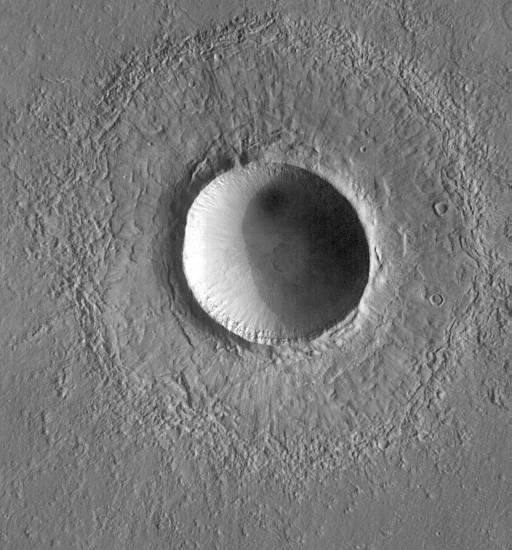
\includegraphics[width=0.166\textwidth]{images/Gre13/Gre13_01.jpg} &
		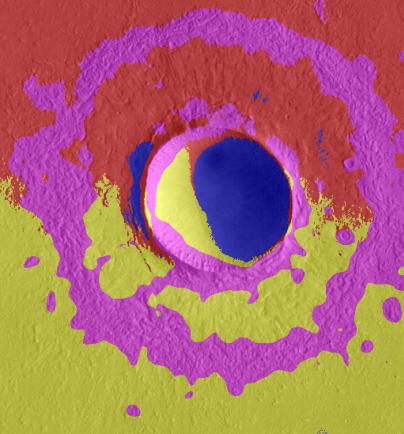
\includegraphics[width=0.166\textwidth]{images/gen/filterbanks/Gre13_01.jpg_TSUGF.png} &
		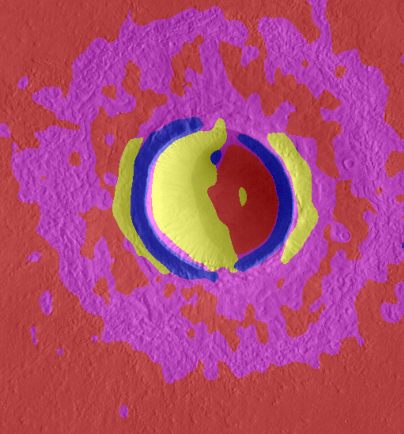
\includegraphics[width=0.166\textwidth]{images/gen/filterbanks/Gre13_01.jpg_LM.png} &
		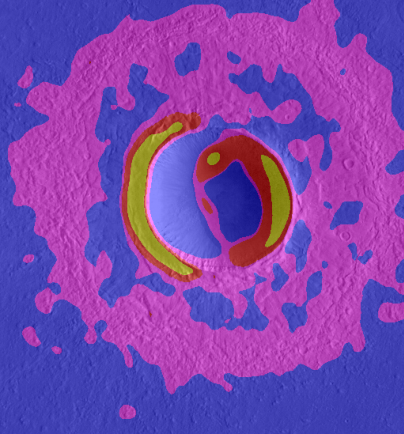
\includegraphics[width=0.166\textwidth]{images/gen/filterbanks/Gre13_01.jpg_S.png} &
		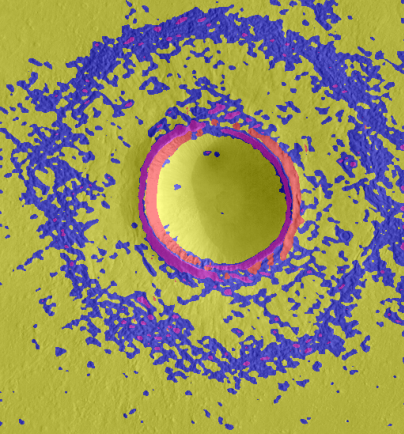
\includegraphics[width=0.166\textwidth]{images/gen/filterbanks/Gre13_01.jpg_MR.png} \\
		
		Vulkan &
		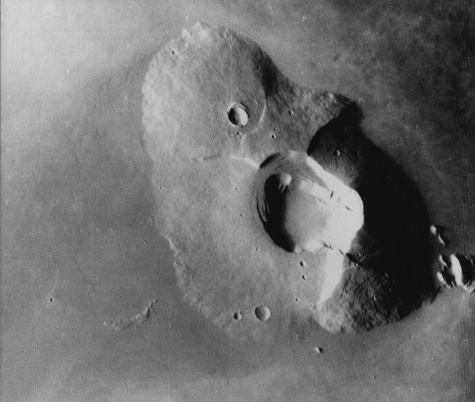
\includegraphics[width=0.166\textwidth]{images/Gre13/Gre13_02.jpg} &
		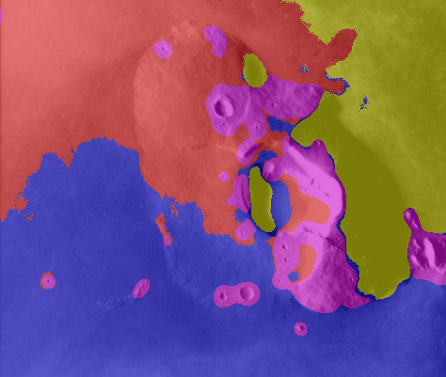
\includegraphics[width=0.166\textwidth]{images/gen/filterbanks/Gre13_02.jpg_TSUGF.png} &
		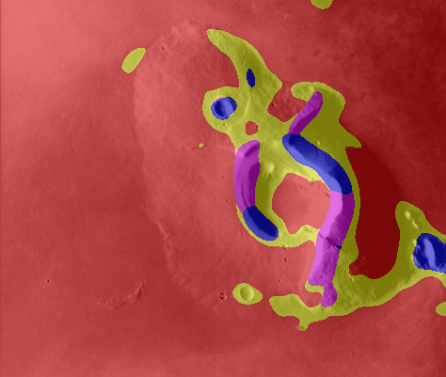
\includegraphics[width=0.166\textwidth]{images/gen/filterbanks/Gre13_02.jpg_LM.png} &
		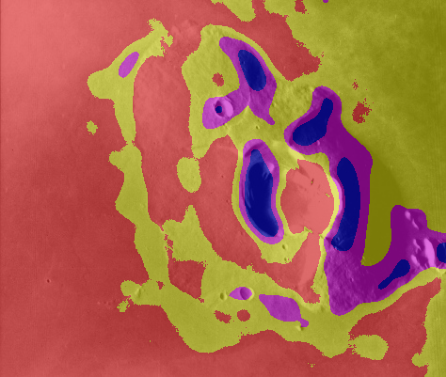
\includegraphics[width=0.166\textwidth]{images/gen/filterbanks/Gre13_02.jpg_S.png} &
		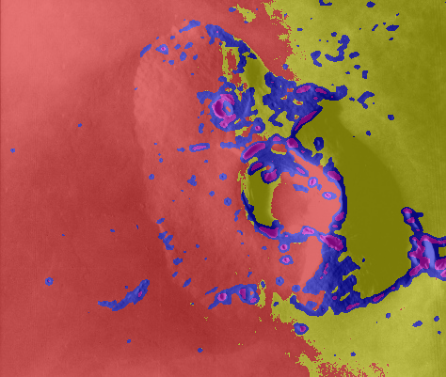
\includegraphics[width=0.166\textwidth]{images/gen/filterbanks/Gre13_02.jpg_MR.png} \\
		
		Vulkan mit\newline strahlen-\newline förmigen Merkmalen &
		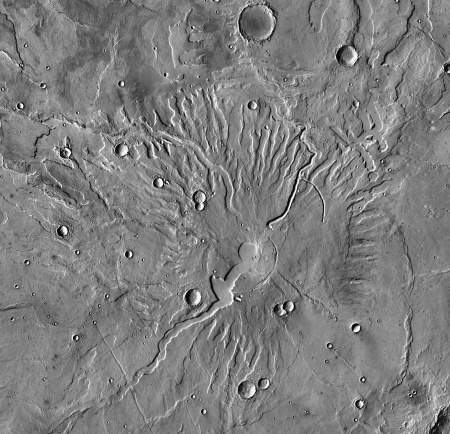
\includegraphics[width=0.166\textwidth]{images/Gre13/Gre13_03.jpg} &
		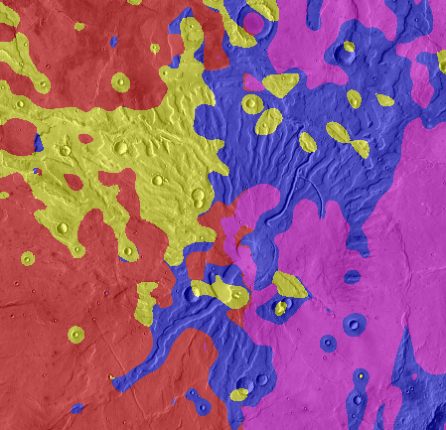
\includegraphics[width=0.166\textwidth]{images/gen/filterbanks/Gre13_03.jpg_TSUGF.png} &
		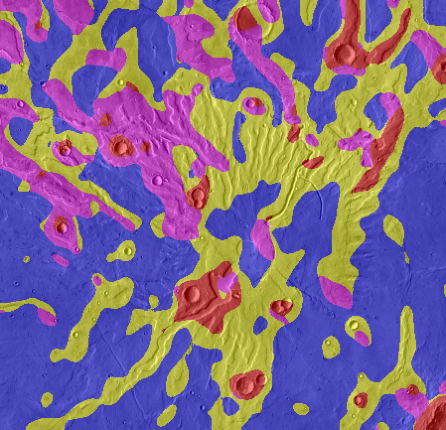
\includegraphics[width=0.166\textwidth]{images/gen/filterbanks/Gre13_03.jpg_LM.png} &
		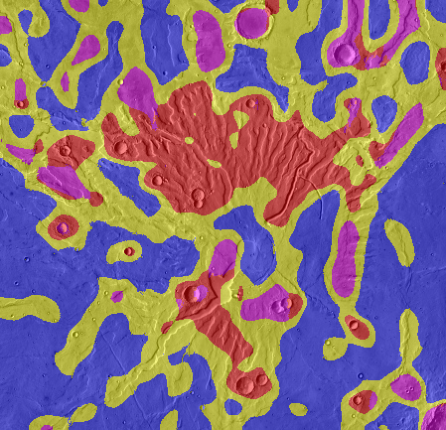
\includegraphics[width=0.166\textwidth]{images/gen/filterbanks/Gre13_03.jpg_S.png} &
		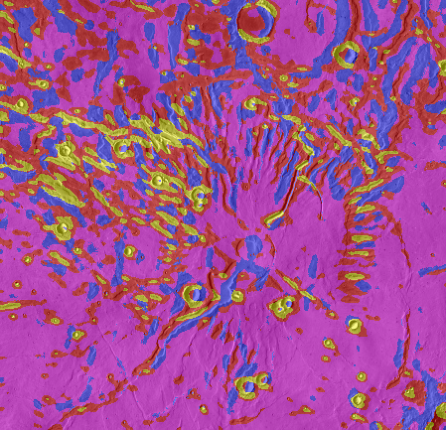
\includegraphics[width=0.166\textwidth]{images/gen/filterbanks/Gre13_03.jpg_MR.png} \\
		
		Gletscher &
		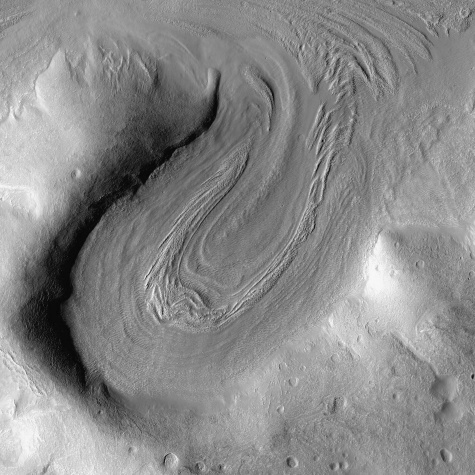
\includegraphics[width=0.166\textwidth]{images/Gre13/Gre13_05.jpg} &
		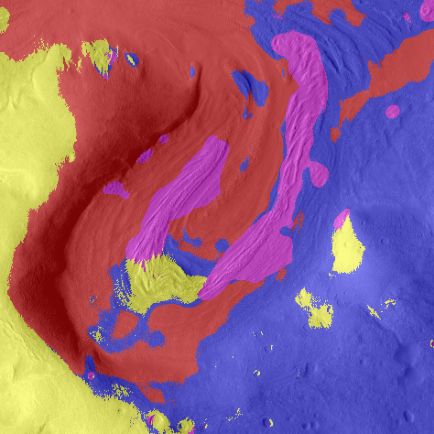
\includegraphics[width=0.166\textwidth]{images/gen/filterbanks/Gre13_05.jpg_TSUGF.png} &
		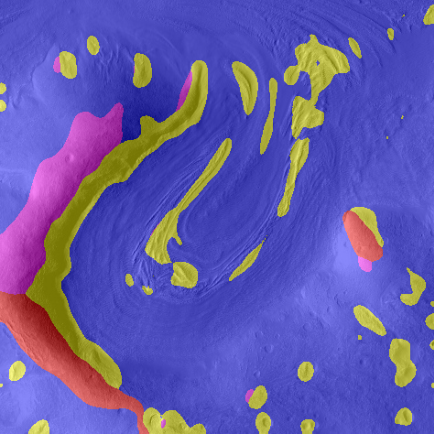
\includegraphics[width=0.166\textwidth]{images/gen/filterbanks/Gre13_05.jpg_LM.png} &
		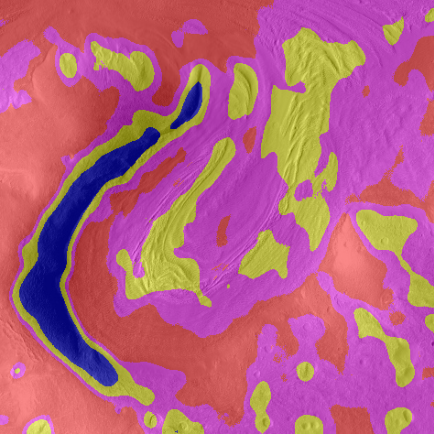
\includegraphics[width=0.166\textwidth]{images/gen/filterbanks/Gre13_05.jpg_S.png} &
		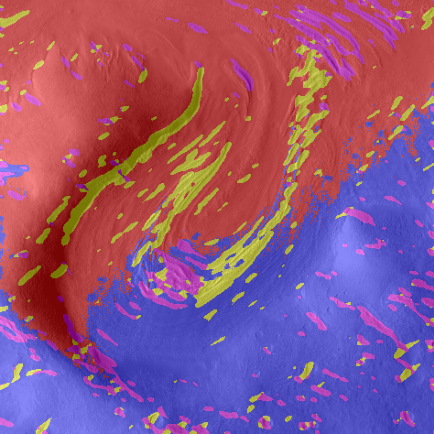
\includegraphics[width=0.166\textwidth]{images/gen/filterbanks/Gre13_05.jpg_MR.png} \\
		
		&
		\hspace{1pt}\newline\centering Eingabe, aus \cite{greeley_13} &
		\hspace{1pt}\newline\centering Filterbank nach \cite{jain_91} &
		\hspace{1pt}\newline\centering LM-Filterbank \cite{leung_01} &
		\hspace{1pt}\newline\centering S-Filterbank \cite{schmid_01} &
		\hspace{1pt}\newline\centering MR-Filterbank \cite{visgeo} \\
	\end{tabular}
	\caption{Vergleich verschiedener Filterbänke auf Bildern der Marsoberfläche. Die Farben der jeweiligen Cluster wurden zufällig gewählt und sagen nichts über deren Inhalt aus. Alle Bilder wurden in vier Cluster eingeteilt.}
	\label{fig:filterbank_comparision}
\end{figure}

\paragraph{Krater}
Neben dem eigentlichen Krater ist auf dieser Aufnahme der Ring aus gröberem Gestein ein wichtiges Merkmal. Dieser wird von allen Filterbänken zuverlässig erkannt, wenn auch mit einer unterschiedlichen Dicke: Die LM- und S-Filterbank selektieren dieses Gestein eher großzügig, die MR-Filterbank hingegen zeigt sehr enge Markierungen dieser Region.

Alle Filterbänke formen einen Ring (oder dessen Ansatz) auf dem Kraterrand, die Maximum Response-Filterbank erzeugt zwei konzentrische Ringe

Der Krater selbst wird von den Filterkombinationen nach \cite{jain_91} und der LM-Filterbank leider nur in Hell- und Dunkel-Regionen aufgeteilt, die S-Filterbank zeigt innerhalb des Kraters kein brauchbares Ergebnis. Eine Ausnahme stellt die Maximum-Response-Filterbank dar, welche neben den zwei erwähnten konzentrischen Clustern den Bereich innerhalb des Kraters als ein einziges Cluster erkennt. Die Maximum Response-Bank erzeugt in diesem Bereich das Resultat, welches sich wohl als bestes zur Weiterverarbeitung eignet.

% TODO Weil...

\paragraph{Vulkan}
Der Vulkanberg wird leider von keiner Filterbank optimal erkannt. Der äußere Rand wird nur von der S-Filterbank als ein Cluster erkannt, dies allerdings nicht sehr genau. Der rauere Bereich der Oberfläche, was kleinere Krater miteinbeschließt, wird vom MR-Filter am ehesten und genausten erkannt, auf dem zweiten Platz folgt die Filterbank nach \cite{jain_91}, welche zwar alle Krater in ein Cluster fügt (violett), allerdings eher gröber.

Die Vulkanmitte wird von keiner Filterbank erkannt, nur bei der MR-Bank lässt sich eine ringförmige, rauere Stelle um den Krater herum erahnen. Die anderen Filterbänke selektieren an dieser Stelle hauptsächlich nach den Helligkeitswerten. Außerdem ist interessant, dass der LM-Filter die Bergspitzen in vom Umfeld getrennte Cluster einteilt (blau und violett). Somit scheint es, als ließe sich diese Aufnahme über keine Filterbank gut clustern. Am ehesten eignet sich allerdings erneut die MR-Bank.

\paragraph{Vulkan mit strahlenförmigen Merkmalen}

Das Ziel bei der Nutzung dieser Marsaufnahme zur Analyse besteht daraus zu analysieren, mit welcher Filterbank die konzentrischen Strahlen am genauesten erkannt werden. Des Weiteren existieren auf der Aufnahme noch Krater, welche es separat einzuordnen gilt.

Die Filterbank nach \cite{jain_91} erkennt die gröberen Strukturen (Strahlen und Krater), fügt diese allerdings in dasselbe Cluster ein (gelb und blau).

Die LM-Filterbank scheint kein brauchbares Ergebnis zu produzieren, sie erkennt im Allgemeinen nur einige der Krater (rot) separat von deren Umfeld, die Strahlen sind nicht geeignet geclustert worden.

Die Schmid-Filterbank clustert einen Großteil der Strahlen gemeinsam in ein Cluster (rot). Die Krater hingegen sind nicht fest einer Clusterart zugewiesen, ein Großteil von ihnen befindet sich jedoch auch im roten Cluster.

Wie in den vorherigen Tests ist das Resultat der MR-Filterbank schon fast zu genau, die Cluster sind sehr fein gehalten. Im Gegensatz zu den Alternativen, werden hier die Krater relativ zuverlässig in gelbe Cluster eingeordnet, die Strahlen sind leider zu fein markiert, als dass man sie getrennt erkennen könnte. Dieses Phänomen könnte sich allerdings in der praktischen Anwendung zunutze gemacht werden, da dafür eine zu feine Initialisierung notwendig ist.

\paragraph{Gletscher}

Der Gletscher stellt im Bereich der Bildsegmentierung ein vergleichsweise schwieriges Problem dar, da er an vielen seiner Ränder keine feste Grenze zu benachbarten Regionen zeigt, nur links auf der Aufnahme ist er durch eine Hügelreihe strikt begrenzt. Diese Grenze wird von allen Filterbänken separat in ein oder mehrere getrennte Cluster unterteilt, mit Ausnahme der Filterbank nach \cite{jain_91}: Diese produziert kein geeignetes Ergebnis, nur die stärker erkennbaren \enquote{Streifen} werden gut erkannt (violett). Die LM-Filterbank erkennt zwar die Abgrenzung auf der linken Seite, allerdings keine anderen Regionen korrekt. Sie liefert bei diesem Bild das wohl schlechteste Resultat. Die Maximum-Response Methode und die Filterbank nach \cite{schmid_01} liefern zwar etwas bessere Ergebnisse, diese sind allerdings nicht ausreichend. Die MR-Bank erzeugt erneut sehr feine Cluster.

\paragraph{}
Zusammengefasst erzeugt aus dieser Auswahl an Filterbänden die Maximum Response-Methode von \cite{visgeo} das wohl am ehesten geeignete Resultat zur Weiterverarbeitung, da sie bei einem Großteil der Beispielbilder das beste Ergebnis produziert hat. Auf dem zweitem Platz folgt die Schmid-Filterbank.

\subsection{Größe der Filter}
\label{ssec:exp_filtersize}

% TODO WTF annotation

Es wird nun versucht, die Ergebnisse der Maximum Response-Filterbank zu verbessern, da diese in vorherigen Versuchen die besten Ergebnisse erzielt hat.

Bis jetzt wurden die Marsaufnahmen aus \cite[Kap.~7]{greeley_13} genutzt, da diese möglichst diverse Oberflächenstrukturen- und Merkmale abdecken. Von dieser Stelle an müssen allerdings Marsaufnahmen genutzt werden, bei denen die Auflösung bekannt ist, somit scheiden die genutzten leider aus. Stattdessen werden Ausschnitte aus der Aufnahme \texttt{P03\_002147\_1865\_XI\_06N208W} der Context Camera des Mars Reconnaissance Orbiters genutzt. Auch diese wurden so ausgewählt, dass sie möglichst diverse Strukturen und Texturen aufweisen. Ein weiterer Vorteil der Nutzung dieser Bilder besteht daraus, dass die Clusteringalgorithmen nun an realitätsnähreren Daten getestet werden können, statt an isolierten Aufnahmen einzelner Besonderheiten der Oberfläche. Die Ergebnisse sind in \figurename~\ref{fig:filterbank_sizes} zu sehen. Als Startwert wurde ein Skalierungsfaktor $s=1$ betrachtet, angewandt auf die vorgestellten, quadratischen Filter mit einer originalen Kantenlänge von \SI{49}{\pixel}.  Dieser wurde nach oben und unten hin in Schritten von $\Delta s=0.25$ verändert, und mit der skalierten MR-Filterbank ein neues Clustering der vier Ausschnitte erstellt. Die Eingabebilder sind quadratisch und besitzen eine Seitenlänge von \SI{650}{\pixel} bei einer Auflösung von \SI{6,17}{\meter\per\pixel}. Jedes der Eingabebilder wurde erneut in vier Bereiche eingeteilt, die Farben sind zur Veranschaulichung zufällig gewählt, da der Algorithmus zwar in Segmente unterteilen kann, allerdings nicht bestimmen kann, was diese Segmente enthalten.

\begin{figure}[h!]
	\setlength\tabcolsep{1pt}
	\def\arraystretch{0.5}
	\begin{tabular}{m{15pt}m{0.14\textwidth}m{0.14\textwidth}m{0.14\textwidth}m{0.14\textwidth}m{0.14\textwidth}m{0.14\textwidth}m{0.14\textwidth}}
		\texttt{a)} &
		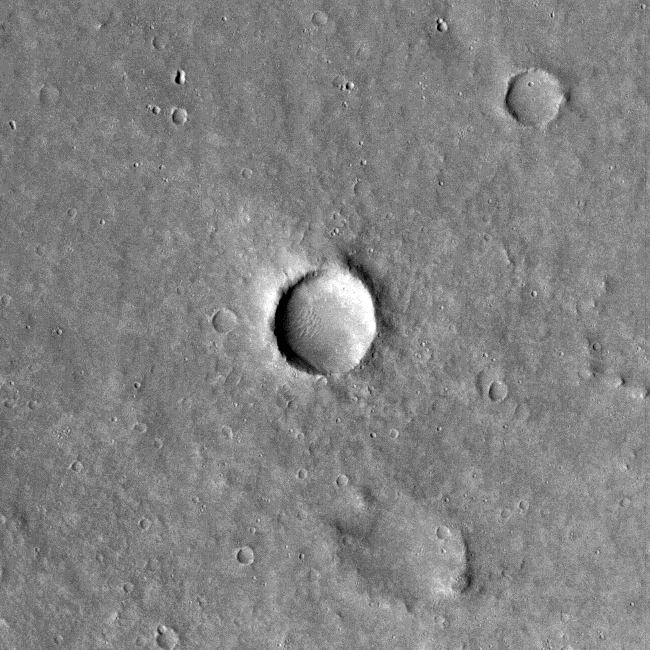
\includegraphics[width=0.14\textwidth]{images/p03/p03_01.png} &
		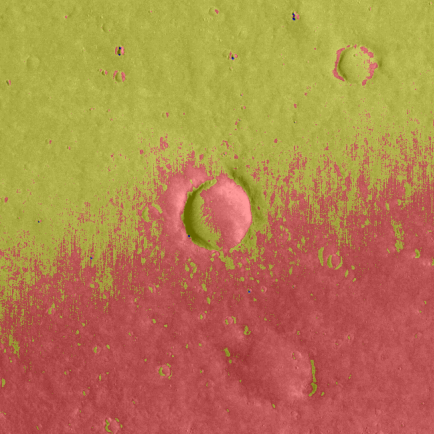
\includegraphics[width=0.14\textwidth]{images/gen/filter_size/p03_01.png_0.25.png} &
		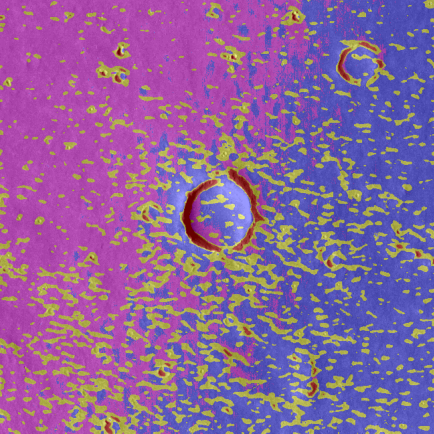
\includegraphics[width=0.14\textwidth]{images/gen/filter_size/p03_01.png_0.50.png} &
		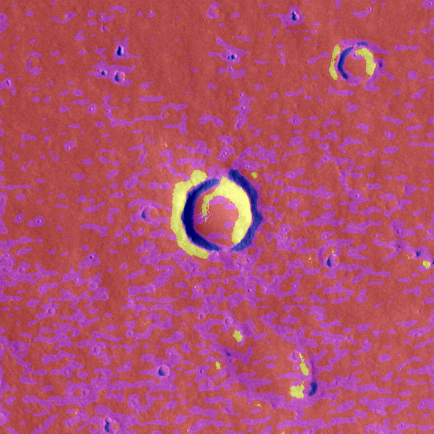
\includegraphics[width=0.14\textwidth]{images/gen/filter_size/p03_01.png_0.75.png} &
		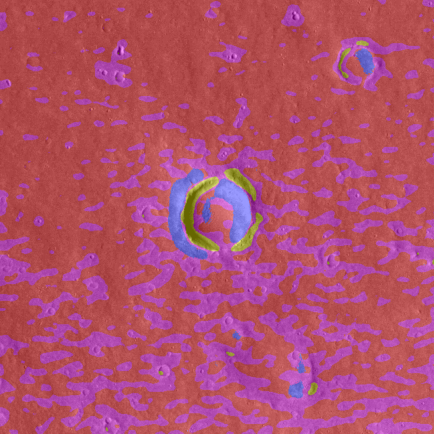
\includegraphics[width=0.14\textwidth]{images/gen/filter_size/p03_01.png_1.00.png} &
		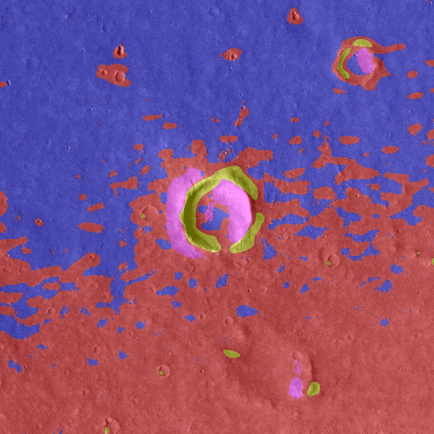
\includegraphics[width=0.14\textwidth]{images/gen/filter_size/p03_01.png_1.25.png} &
		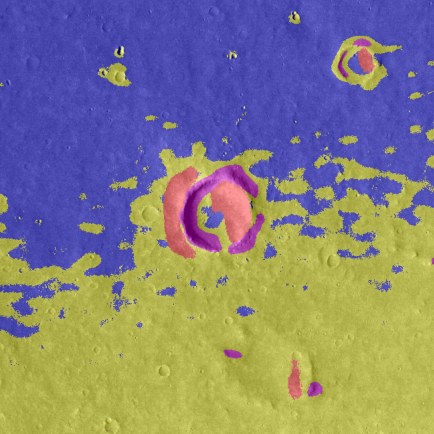
\includegraphics[width=0.14\textwidth]{images/gen/filter_size/p03_01.png_1.50.png} \\
		\texttt{b)} &
		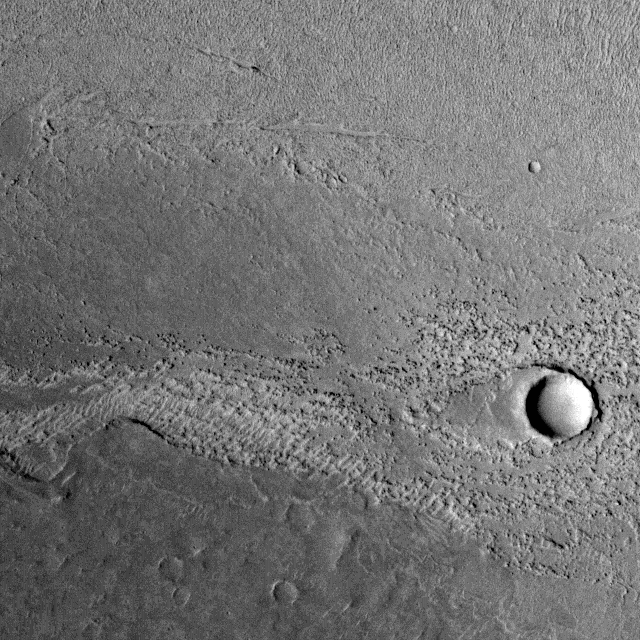
\includegraphics[width=0.14\textwidth]{images/p03/p03_02.png} &
		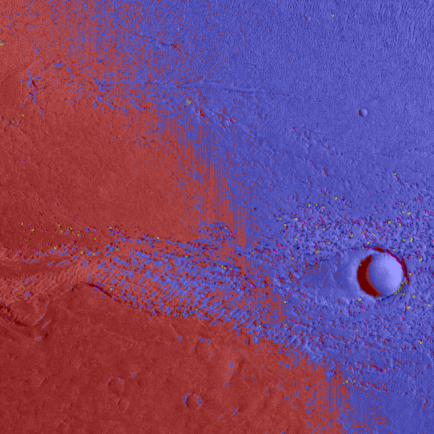
\includegraphics[width=0.14\textwidth]{images/gen/filter_size/p03_02.png_0.25.png} &
		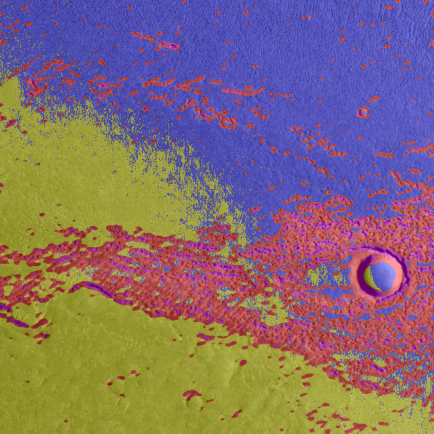
\includegraphics[width=0.14\textwidth]{images/gen/filter_size/p03_02.png_0.50.png} &
		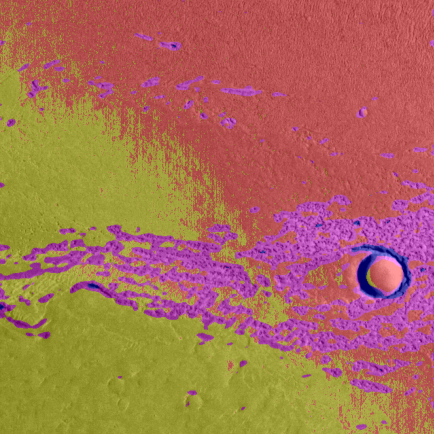
\includegraphics[width=0.14\textwidth]{images/gen/filter_size/p03_02.png_0.75.png} &
		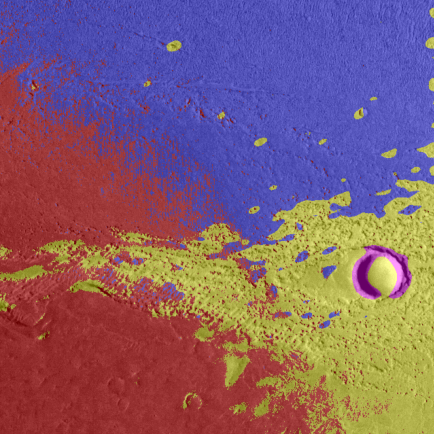
\includegraphics[width=0.14\textwidth]{images/gen/filter_size/p03_02.png_1.00.png} &
		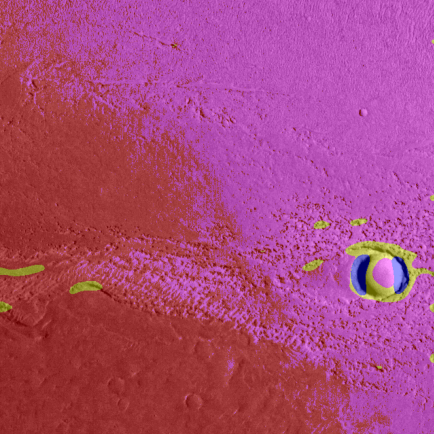
\includegraphics[width=0.14\textwidth]{images/gen/filter_size/p03_02.png_1.25.png} &
		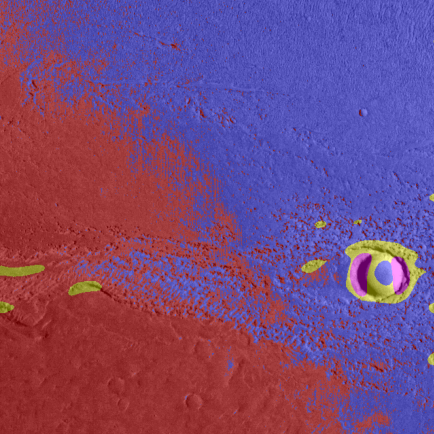
\includegraphics[width=0.14\textwidth]{images/gen/filter_size/p03_02.png_1.50.png} \\
		\texttt{c)} &
		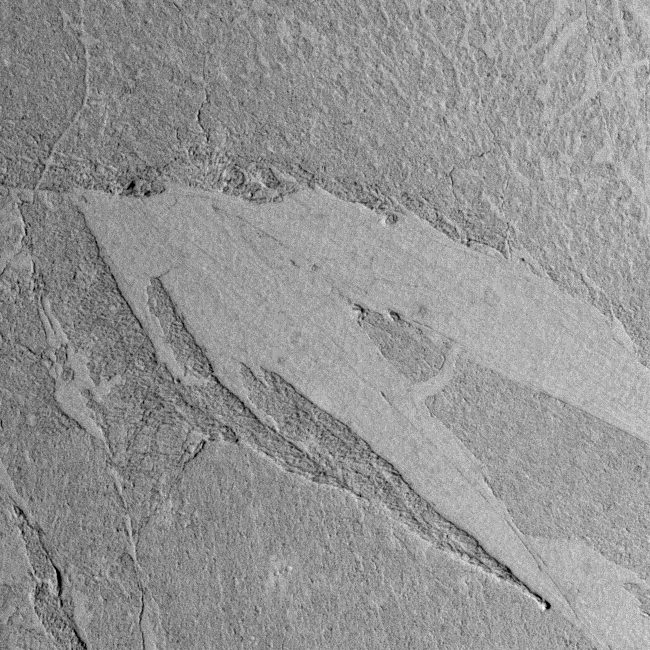
\includegraphics[width=0.14\textwidth]{images/p03/p03_03.png} &
		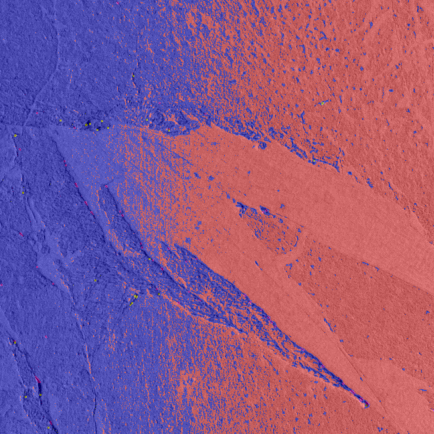
\includegraphics[width=0.14\textwidth]{images/gen/filter_size/p03_03.png_0.25.png} &
		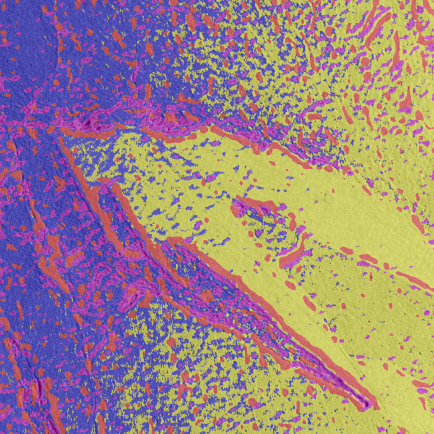
\includegraphics[width=0.14\textwidth]{images/gen/filter_size/p03_03.png_0.50.png} &
		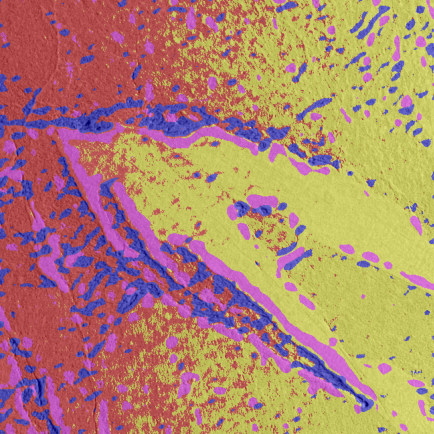
\includegraphics[width=0.14\textwidth]{images/gen/filter_size/p03_03.png_0.75.png} &
		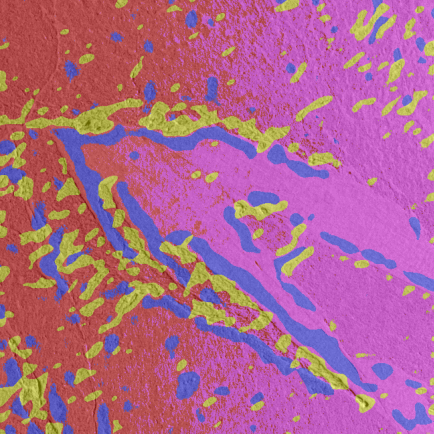
\includegraphics[width=0.14\textwidth]{images/gen/filter_size/p03_03.png_1.00.png} &
		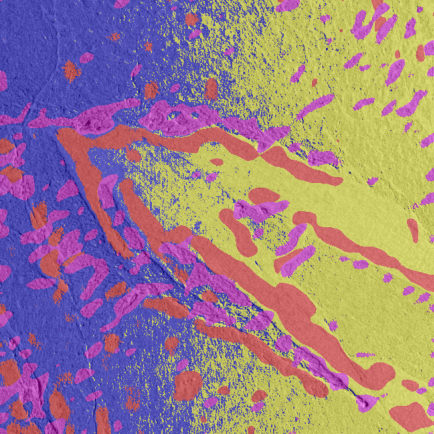
\includegraphics[width=0.14\textwidth]{images/gen/filter_size/p03_03.png_1.25.png} &
		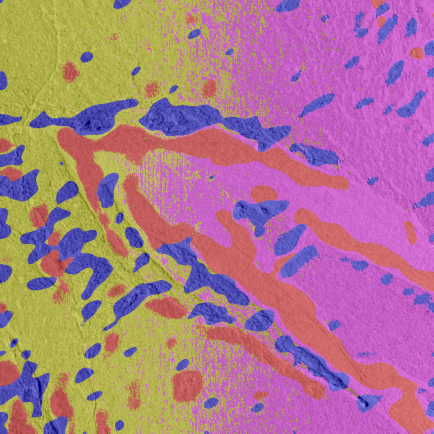
\includegraphics[width=0.14\textwidth]{images/gen/filter_size/p03_03.png_1.50.png} \\
		\texttt{d)} &
		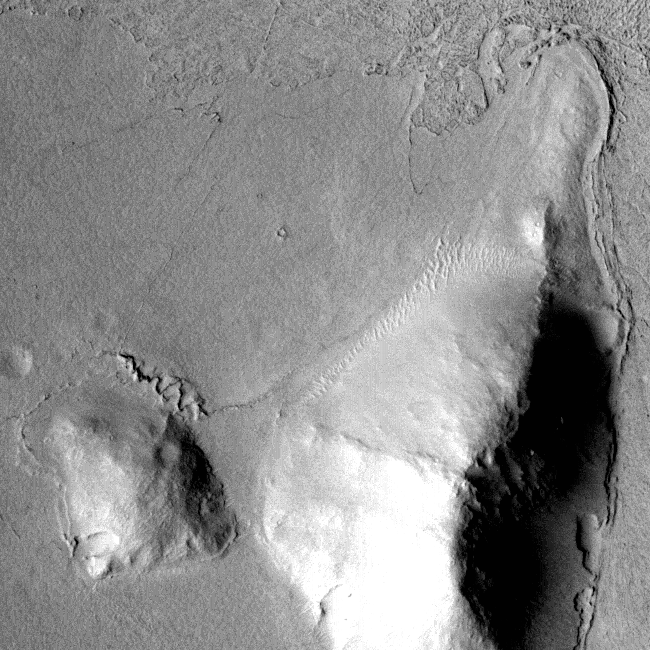
\includegraphics[width=0.14\textwidth]{images/p03/p03_04.png} &
		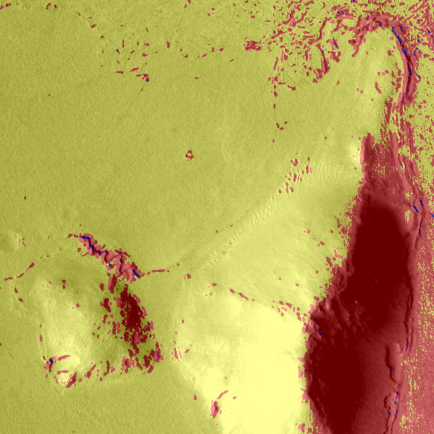
\includegraphics[width=0.14\textwidth]{images/gen/filter_size/p03_04.png_0.25.png} &
		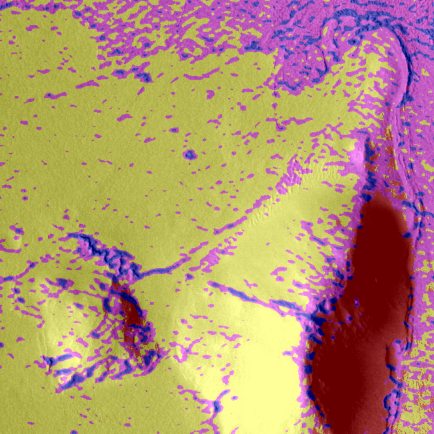
\includegraphics[width=0.14\textwidth]{images/gen/filter_size/p03_04.png_0.50.png} &
		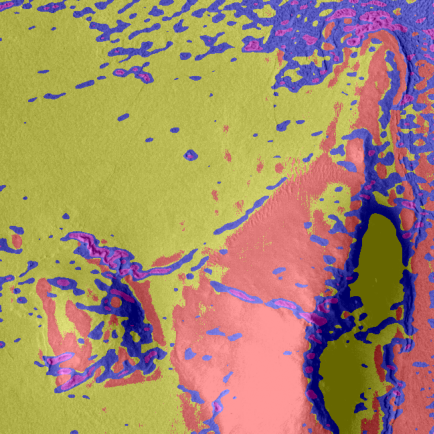
\includegraphics[width=0.14\textwidth]{images/gen/filter_size/p03_04.png_0.75.png} &
		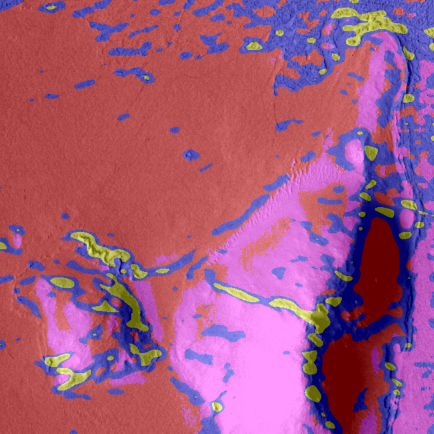
\includegraphics[width=0.14\textwidth]{images/gen/filter_size/p03_04.png_1.00.png} &
		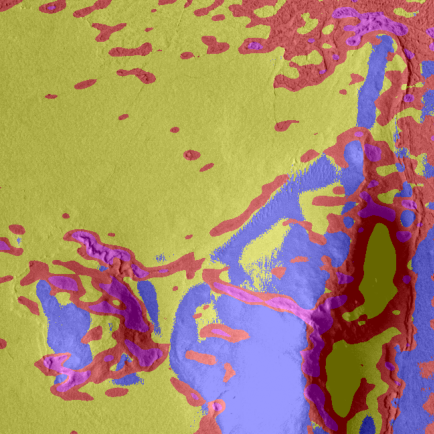
\includegraphics[width=0.14\textwidth]{images/gen/filter_size/p03_04.png_1.25.png} &
		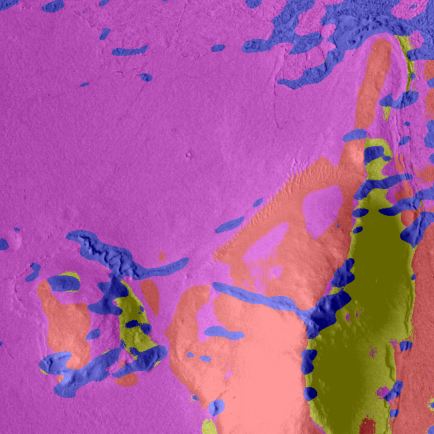
\includegraphics[width=0.14\textwidth]{images/gen/filter_size/p03_04.png_1.50.png} \\
		
		&
		\hspace{2pt}\newline\centering Eingabe & 
		\hspace{2pt}\newline\centering $s=0,25$ &
		\hspace{2pt}\newline\centering $s=0,50$ &
		\hspace{2pt}\newline\centering $s=0,75$ &
		\hspace{2pt}\newline\centering $s=1,00$ &
		\hspace{2pt}\newline\centering $s=1,25$ &
		\hspace{2pt}\newline\centering $s=1,50$
	\end{tabular}
	\caption{Vergleich verschiedener Skalierungen der MR-Filterbank auf Bildern der Marsoberfläche. Die Farben der jeweiligen Cluster wurden zufällig gewählt und sagen nichts über deren Inhalt aus. Alle Bilder wurden in vier Cluster eingeteilt.}
	\label{fig:filterbank_sizes}
\end{figure}

Von hier an gilt in allen Vergleichen von Segmentierungen: Die erste Zeile der Tabelle entspricht der ersten Aufnahme, die zweile Zeile entspricht der Zweiten Aufnahme, \etc.

\paragraph{Skalierungsfaktor $s=0,25$}

Auf Aufnahme \texttt{a)} ist, vergleichbar mit den Beispielaufnahmen aus dem letzten Abschnitt, ein runder Krater zentriert zu sehen. Die geringe Skalierung mit dem Faktor $s=0.25$ führt dazu, dass die jeweiligen Filter zu klein sind, um die Strukturen der Oberfläche zu erkennen, somit sieht diese Aufnahme aus, als wäre nur anhand ihrer Helligkeitswerten geclustert worden. Das gleiche gilt auch für die Aufnahmen \texttt{b)} und \texttt{d)}.

Aufnahme \texttt{c)} stellt eine relativ ebenmäßige Fläche in einem Umfeld von gröberer Oberfläche dar. Dort scheint es, als gäbe es nicht genug Kontrast um nach den Helligkeitswerten zu clustern, der Algorithmus erstellt eine Filterung anhand der X- und Y-Koordinaten. Bei allen Aufnahmen werden nur zwei wirkliche Cluster erstellt, die letzten zwei Cluster die erstellt werden sollten bestehen nur aus jeweils wenigen Pixeln.

Dieser Skalierungsfaktor produziert keine brauchbaren Ergebnisse.

\paragraph{Skalierungsfaktor $s=0,50$}

Wie zu Erwarten führt die genutzte, noch relativ geringe Skalierung der Filterbank mit $s=0,50$ zu vielen kleineren Clustern, in diesem Fall auf Aufnahme \texttt{a)} deutlich erkennbar anhand der gelb markierten Flächen. Obwohl es auf den ersten Blick scheint, als würden die Kraterränder erkannt werden, werden durch die Filterbank bei dieser Skalierung nur die dunkleren Bereiche, in diesem Fall die Schatten, welche die erhöhten Kraterränder werfen, erkannt. Auf dieser Aufnahme führt dies zwar zu einer vergleichsweise guten Approxmimation der Krater, sobald anderweitige Schatten hinzukommen, produziert diese Skalierung allerdings keine geeigneten Resultate.

Das selbe Phänomen tritt bei der Aufnahme in der zweiten Zeile von oben auf, auch dort wird stark anhand der Helligkeitswerte geclustert, erkennbar insbesondere an den violetten Bereichen an den Kraterrändern. Bei diesem Bild wird allerdings auch trotz der kleineren Skalierung das raue Gebiet, welches sich horizontal durch das Bild erstreckt, in ein (rot gefärbtes) Cluster eingeteilt. Auch hier werden allerdings dunklerere Bereiche (wie die Kraterränder) in separate (violett gefärbte) Cluster eingeteilt.

Auf Aufnahme \texttt{c)} wird bei der genutzten Skalierung die feinere Fläche größtenteils als ein (gelb gefärbtes) Cluster dargestellt, separat dazu sind in rot die Übergänge zwischen den Regionen gekennzeichnet. Die gröberen Flächen in den äußeren Bereichen werden nicht zuverlässig in das selbe Cluster eingeordnet.

Die letzte Testaufnahme, bestehend aus zwei Hügeln \bzw Bergen, stellt durch die stark und wenig belichteten Flächen an den Hängen eine der größten Herausforderungen für den Clusteringalgorithmus dar. An diesen Stellen ist der Kontrast des Bildes sehr gering, sodass kaum noch Texturen erkannt werden, anhand derer geclustert werden könnte. Wie zu erwarten werden die dunklen Flächen in ein einzelnes (rotes) Cluster kombiniert. Kleine Hügelketten hingegen werden zuverlässig in zusammengehörige Cluster eingeteilt, welches auf diesen Aufnahmen blau markiert ist. Die beleuchteten Seiten der Hügel werden bei dieser Skalierung leider nicht von der allgemeinen Marsoberfläche unterschieden, höchstens der Fuß des Berges kann durch die violette Färbung erahnt werden.

Dieser Skalierungsfaktor führt zu vergleichsweise guten Clusteringergebnissen.

\paragraph{Skalierungsfaktor $s=0,75$}

Dieser Skalierungsfaktor führt beim Clustering des obersten Bildes, Aufnahme \texttt{a)}, zu Resultaten, welche vergleichbar mit denen des Faktors $s=0,5$ sind. Die Ränder der Krater werden allerdings getrennt in helle und dunkle Regionen eingeteilt, die Cluster im äußeren Bereich sind größer und gröber.

Auf Aufnahme \texttt{b)} wird die horizontale rauere Region sehr gut in ein eigenes Cluster eingeteilt, selbiges gilt für die Kraterränder. Auf dieser Aufnahme erscheint der Skalierungsfaktor $s=0,75$ für diese Filterbank optimal.

Die vorletzte Aufnahme, Aufnahme \texttt{c)}, unterscheidet sich bis auf die gröberen, größeren Cluster in den äußeren Bereichen nicht wesentlich von der vorherigen Skalierung.

Bei der untersten Aufnahme führt die größere Skalierung zu einem uniformen Clusterings des beleuchteten Berghangs, er wird als eine große Fläche erkannt. Die dunkle Seite hingegen wird in zwei Cluster unterteilt: Die eigentliche dunkle Seite des Berges, und die Stellen, welche zu unterbelichtet sind, um aus ihnen eine Textur zu erkennen.

Insgesamt scheint sich dieser Skalierungsfaktor auch zum texturbasierten Clustering zu eignen.

\paragraph{Skalierungsfaktor $s=1.00$}

Während bei diesem Skalierungsfaktor auf Aufnahme \texttt{a)} der größere, mittige Krater relativ gut durch ein gelbes kreisförmiges Cluster gekennzeichnet wird, wird der kleinere Krater nicht zuverlässig erkannt. Bei diesem gehen die Cluster in umlegende Gebiete über, als wäre dieser Krater nur eine etwas rauere Oberflächenstruktur.

Bei Aufnahme \texttt{b)} wird wie zuvor der Krater erfolgreich separat in ein Cluster eingeteilt, die Begrenzungen der gröberen Struktur, welche sich durch das Bild zieht, geht allerdings verloren. Diese Region wird leider im rechten Teil des Bildes sehr weitläufig erkannt.

In Testbild \texttt{c)} werden die gröberen Hügelketten am Rand des helleren Bereiches zwar erkannt (gelb markiert), und die Übergangsstellen zwischen zwei Regionen werden in ein blaues Cluster zusammengefügt, alle anderen Regionen sind allerdings nicht voneinander getrennt worden.

Bild \texttt{d)} wird bei dieser Skalierung fast identisch zu der Skalierung mit $s=0,75$ geclustert.

Zusammengefasst ist diese Skalierung schon zu grob um so gute Ergebnisse wie die vorherigen zu erreichen.

\paragraph{Skalierungsfaktor $s=1.25$ und $s=1.50$}

Da diese beiden Skalierungsfaktoren zu fast identischen Clusterverteilungen führen, werden sie in einen Abschnitt zusammengefasst.

Bei diesen Skalierungen werden im oberen, weniger rauen Bereich der Aufnahme \texttt{a)} die vereinzelten Krater wie gewollt erkannt, sie versagt allerdings im unteren, gröberen Bereich, wo sie nur ein großes Cluster erstellen. Der Krater wird nur anhand von starken Helligkeitsdifferenzen erkannt, welche in der gesamten Ausgabe gelb bei $s=1,25$, \bzw violett bei $s=1,5$ markiert wurden. 

Selbiges gilt im Bezug auf die starken Helligkeitsdifferenzen in Aufnahme \texttt{b)}.

Bei Aufnahme \texttt{c)} wird von beiden Skalierungsfaktoren kein brauchbares Resultat produziert, man kann höchstens erahnen, dass die gelb \bzw violett gefärbten Regionen besonders kontrastarme, also glatte Flächen darstellen sollen.

Beim Clusteringergebnis der letzten Aufnahme unterschieden sich die beiden Skalierungsfaktoren erstmals stärker: Bei $s=1,25$ gleicht das Ergebnis dem des vorherigen Clusterings: Kleinere Bergregionen und rauere Oberflächenstrukturen werden getrennt voneinander erkannt, Flächen mit weniger oder (aufgrund von Unterbelichtung) keiner werden auch in ein großes Cluster hinzugefügt. Der Faktor $s=1,5$ scheint selbst bei diesem Bild zu groß zu sein, bis auf die Hügelketten mit starker Helligkeitsdifferenz wird die Aufnahme nur anhand ihrer Helligkeitswerte geclustert.

Diese Skalierungsfaktoren führen also zu Filtern, welche eine zu große Kantenlänge besitzen um brauchbare Resultate zu produzieren, da die Muster innerhalb einer Oberflächentextur eine wesentlich geringere Entfernung besitzen, nach welcher sie sich wiederholen.

\paragraph{}
Aus diesen Ergebnissen lässt sich schlussfolgern, dass sich die Skalierungsfaktoren $s=0,5$ und $s=0,75$ bei diesen Eingabedaten die besten Resultate liefert. Da durch die nachfolgende Weiterverarbeitung durch den Algorithmus nach Kanezaki eine hohe Anzahl an Clustern benötigt wird, diese aber nicht zu klein und verstreut ausfallen sollten, wird von nun an ein Skalierungsfaktor von $s=0,75$ genutzt.

\subsection{Gewichtung der Parameter}
\label{ssec:exp_filterweight}

Wie in Unterabschnitt~\ref{ssec:initialization_filterweight} erläutert, spielt die Gewichtung der Komponenten des Datenwürfels, welcher zum Clustering durch k-Means genutzt wird eine wichtige Rolle. In den Abbildungen~\ref{fig:filterbank_weights_pos} und \ref{fig:filterbank_weights_col} die Resultate des Clusterings mit unterschiedlichen Werten für diese jeweiligen Gewichtungen zu sehen. Die Skalierung der Filter beträgt $s=0,5$, da im vorherigen Unterabschnitt festgestellt wurde, dass dieser Wert relativ gute Ergebnisse liefert.

\begin{figure}[h!]
	\setlength\tabcolsep{1pt}
	\def\arraystretch{0.5}
	\begin{tabular}{m{15pt}m{0.14\textwidth}m{0.14\textwidth}m{0.14\textwidth}m{0.14\textwidth}m{0.14\textwidth}m{0.14\textwidth}m{0.14\textwidth}}
		\texttt{a)} &
		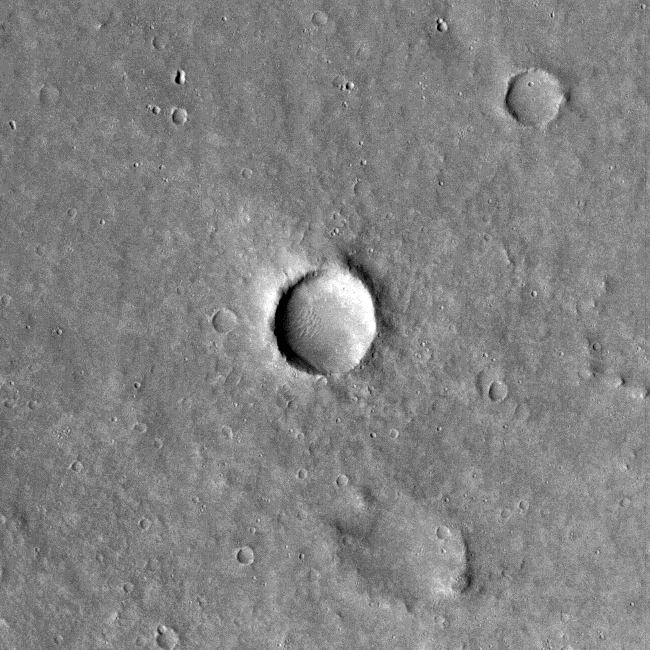
\includegraphics[width=0.14\textwidth]{images/p03/p03_01.png} &
		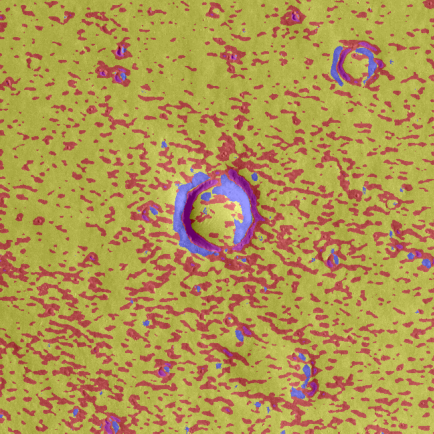
\includegraphics[width=0.14\textwidth]{images/gen/spatial_weight/p03_01.png_0.00.png} &
		\includegraphics[width=0.14\textwidth]{images/gen/spatial_weight/p03_01.png_0.33.png} &
		\includegraphics[width=0.14\textwidth]{images/gen/spatial_weight/p03_01.png_0.66.png} &
		\includegraphics[width=0.14\textwidth]{images/gen/spatial_weight/p03_01.png_1.00.png} &
		\includegraphics[width=0.14\textwidth]{images/gen/spatial_weight/p03_01.png_1.33.png} &
		\includegraphics[width=0.14\textwidth]{images/gen/spatial_weight/p03_01.png_1.66.png} \\
		\texttt{b)} &
		\includegraphics[width=0.14\textwidth]{images/p03/p03_02.png} &
		\includegraphics[width=0.14\textwidth]{images/gen/spatial_weight/p03_02.png_0.00.png} &
		\includegraphics[width=0.14\textwidth]{images/gen/spatial_weight/p03_02.png_0.33.png} &
		\includegraphics[width=0.14\textwidth]{images/gen/spatial_weight/p03_02.png_0.66.png} &
		\includegraphics[width=0.14\textwidth]{images/gen/spatial_weight/p03_02.png_1.00.png} &
		\includegraphics[width=0.14\textwidth]{images/gen/spatial_weight/p03_02.png_1.33.png} &
		\includegraphics[width=0.14\textwidth]{images/gen/spatial_weight/p03_02.png_1.66.png} \\
		\texttt{c)} &
		\includegraphics[width=0.14\textwidth]{images/p03/p03_03.png} &
		\includegraphics[width=0.14\textwidth]{images/gen/spatial_weight/p03_03.png_0.00.png} &
		\includegraphics[width=0.14\textwidth]{images/gen/spatial_weight/p03_03.png_0.33.png} &
		\includegraphics[width=0.14\textwidth]{images/gen/spatial_weight/p03_03.png_0.66.png} &
		\includegraphics[width=0.14\textwidth]{images/gen/spatial_weight/p03_03.png_1.00.png} &
		\includegraphics[width=0.14\textwidth]{images/gen/spatial_weight/p03_03.png_1.33.png} &
		\includegraphics[width=0.14\textwidth]{images/gen/spatial_weight/p03_03.png_1.66.png} \\
		\texttt{d)} &
		\includegraphics[width=0.14\textwidth]{images/p03/p03_04.png} &
		\includegraphics[width=0.14\textwidth]{images/gen/spatial_weight/p03_04.png_0.00.png} &
		\includegraphics[width=0.14\textwidth]{images/gen/spatial_weight/p03_04.png_0.33.png} &
		\includegraphics[width=0.14\textwidth]{images/gen/spatial_weight/p03_04.png_0.66.png} &
		\includegraphics[width=0.14\textwidth]{images/gen/spatial_weight/p03_04.png_1.00.png} &
		\includegraphics[width=0.14\textwidth]{images/gen/spatial_weight/p03_04.png_1.33.png} &
		\includegraphics[width=0.14\textwidth]{images/gen/spatial_weight/p03_04.png_1.66.png} \\
		
		&
		\hspace{2pt}\newline\centering Eingabe & 
		\hspace{2pt}\newline\centering $w_p=0,00$ &
		\hspace{2pt}\newline\centering $w_p=0,33$ &
		\hspace{2pt}\newline\centering $w_p=0,66$ &
		\hspace{2pt}\newline\centering $w_p=1,00$ &
		\hspace{2pt}\newline\centering $w_p=1,33$ &
		\hspace{2pt}\newline\centering $w_p=1,66$
	\end{tabular}
	\caption{Vergleich verschiedener Gewichtungen der Koordinaten beim Clustering der jeweiligen Eingabedateien. Die Farben der jeweilgen Cluster wurden zufällig gewählt. Alle Bilder wurden in vier Cluster eingeteilt.}
	\label{fig:filterbank_weights_pos}
\end{figure}

\paragraph{Gewichtung der Koordinaten}
Das Hinzufügen der X- und Y-Koordinaten zu dem Datenwürfel ist ursprünglich aus dem Grund geschehen, dass ein gegebener räumlicher Bezug zwischen unterschiedlichen Pixeln beim Clustering berücksichtigt werden kann (\vgl Unterabschnitt~\ref{ssec:tsugf}; \cite{jain_91}). Aus den Clusteringergebnissen in \figurename~\ref{fig:filterbank_weights_pos} allerdings lässt sich erkennen, dass dieser räumliche Bezug in diesem Anwendungsfall nicht außerordentlich hilfreich ist: Bei einer Gewichtung von $w_p\geq1,33$ lässt sich eindeutig erkennen, dass der allgemeine Bodenbereich auf allen Aufnahmen zu stark anhand seiner Positionen eingeteilt wird, es entstehen Cluster in den Ecken der Aufnahmen, welche sich ins Zentrum erstrecken. Unter diesem starken Einfluss nimmt zusätzlich die relative Wichtigkeit der ähnlichen Textur ab.

Wird nun ein geringerer Wert für $w_p$ betrachtet, so erkennt man für Werte mit $w_p\leq0,66$ keinen Starken Unterschied bei wechselnden Gewichtungen. Dies ist insbesondere bei $w_p=0$ signifikant, da dort der räumliche Bezug der einzelnen Pixel zueinander bei der Berechnung des Clusterings zwar komplett ignoriert wird, das eigentliche Ergebnis sich, bis auf etwas kleinere Cluster in den merkmalsarmen Bereichen, aber kaum verändert. Dies lässt sich darauf zurückführen, dass das Hinzufügen des räumlichen Bezuges ursprünglich den Grund hatte, dass auf \enquote{normalen} Fotografien die vorkommenden Cluster meistens nur ein einziges mal an einem räumlich begrenzten Ort vorhanden sind, so sind \zB bei der Aufnahme aus \figurename~\ref{fig:tsugf_optim} aus Unterabschnitt~\ref{ssec:tsugf} die kleineren Korallen im linken Hintergrund nur an dieser Stelle vorhanden und ließen sich durch ein weit ausgedehntes Cluster zusammenfassen. Bei den aktuell genutzten Aufnahmen hingegen ist dies nicht der Fall, eine auftretende Oberflächenstruktur, wie \zB ein Krater kann an verschieden Stellen ohne räumlichen Bezug zueinander auftreten.
Die Nutzung der Positionwerte hat allerdings einen Vorteil: Sie sorgt dafür die Clustergrößen nicht zu klein und fragmentiert werden zu lassen, indem sie eine Relation mit benachbarten Pixeln erzeugt, welche der k-Means Algorithmus berücksichtigt.

Aus diesem Grund macht es Sinn, die Koordinatenbeträge der Pixel relativ gering zu gewichten, um dafür zu sorgen, dass das texturbasierte Clustering möglicht positionsinvariant operiert, aber auch nicht so gering, dass viele fragmentierte Cluster entstehen. Anhand von \figurename~\ref{fig:filterbank_weights_pos} ist erkennbar, dass ein Wert von  $w_p=0,66$ sich in diesem Fall sehr gut eignet, ein brauchbares Clusterergebnis zu erstellen.

\paragraph{Gewichtungen der Farb-/Helligkeitswerte}
Die hier folgenden Clusteringergebnisse wurden mit einem Skalierungsfaktor von $s=0,5$ und einer Gewichtung von $w_p=0,66$ für die Positionswerte erstellt.

In der originalen Ausarbeitung des texturbasierten Clusterings \cite{jain_91} werden nur zwei Ebenen für die jeweiligen X- und Y-Koordinaten hinzugefügt. Es steht also an dieser Stelle offen, ob das Hinzufügen der Farb- \bzw Helligkeitsdimension zum Datenwürfel zu besseren Ergebnissen führt. Dazu wurde der vorgestellte Algorithmus mit unterschiedlichen Werten für die Gewichtung der Helligkeitswerte $w_c$ auf den bekannten Beispielbildern ausgeführt. Die Resultate dieses Experimentes sind in \figurename~\ref{fig:filterbank_weights_col} dargestellt.

\begin{figure}[h!]
	\setlength\tabcolsep{1pt}
	\def\arraystretch{0.5}
	\begin{tabular}{m{15pt}m{0.14\textwidth}m{0.14\textwidth}m{0.14\textwidth}m{0.14\textwidth}m{0.14\textwidth}m{0.14\textwidth}m{0.14\textwidth}}
		\texttt{a)} &
		\includegraphics[width=0.14\textwidth]{images/p03/p03_01.png} &
		\includegraphics[width=0.14\textwidth]{images/gen/color_weight/p03_01.png_0.00.png} &
		\includegraphics[width=0.14\textwidth]{images/gen/color_weight/p03_01.png_0.33.png} &
		\includegraphics[width=0.14\textwidth]{images/gen/color_weight/p03_01.png_0.66.png} &
		\includegraphics[width=0.14\textwidth]{images/gen/color_weight/p03_01.png_1.00.png} &
		\includegraphics[width=0.14\textwidth]{images/gen/color_weight/p03_01.png_1.33.png} &
		\includegraphics[width=0.14\textwidth]{images/gen/color_weight/p03_01.png_1.66.png} \\
		\texttt{b)} &
		\includegraphics[width=0.14\textwidth]{images/p03/p03_02.png} &
		\includegraphics[width=0.14\textwidth]{images/gen/color_weight/p03_02.png_0.00.png} &
		\includegraphics[width=0.14\textwidth]{images/gen/color_weight/p03_02.png_0.33.png} &
		\includegraphics[width=0.14\textwidth]{images/gen/color_weight/p03_02.png_0.66.png} &
		\includegraphics[width=0.14\textwidth]{images/gen/color_weight/p03_02.png_1.00.png} &
		\includegraphics[width=0.14\textwidth]{images/gen/color_weight/p03_02.png_1.33.png} &
		\includegraphics[width=0.14\textwidth]{images/gen/color_weight/p03_02.png_1.66.png} \\
		\texttt{c)} &
		\includegraphics[width=0.14\textwidth]{images/p03/p03_03.png} &
		\includegraphics[width=0.14\textwidth]{images/gen/color_weight/p03_03.png_0.00.png} &
		\includegraphics[width=0.14\textwidth]{images/gen/color_weight/p03_03.png_0.33.png} &
		\includegraphics[width=0.14\textwidth]{images/gen/color_weight/p03_03.png_0.66.png} &
		\includegraphics[width=0.14\textwidth]{images/gen/color_weight/p03_03.png_1.00.png} &
		\includegraphics[width=0.14\textwidth]{images/gen/color_weight/p03_03.png_1.33.png} &
		\includegraphics[width=0.14\textwidth]{images/gen/color_weight/p03_03.png_1.66.png} \\
		\texttt{d)} &
		\includegraphics[width=0.14\textwidth]{images/p03/p03_04.png} &
		\includegraphics[width=0.14\textwidth]{images/gen/color_weight/p03_04.png_0.00.png} &
		\includegraphics[width=0.14\textwidth]{images/gen/color_weight/p03_04.png_0.33.png} &
		\includegraphics[width=0.14\textwidth]{images/gen/color_weight/p03_04.png_0.66.png} &
		\includegraphics[width=0.14\textwidth]{images/gen/color_weight/p03_04.png_1.00.png} &
		\includegraphics[width=0.14\textwidth]{images/gen/color_weight/p03_04.png_1.33.png} &
		\includegraphics[width=0.14\textwidth]{images/gen/color_weight/p03_04.png_1.66.png} \\
		
		&
		\hspace{2pt}\newline\centering Eingabe & 
		\hspace{2pt}\newline\centering $w_c=0,00$ &
		\hspace{2pt}\newline\centering $w_c=0,33$ &
		\hspace{2pt}\newline\centering $w_c=0,66$ &
		\hspace{2pt}\newline\centering $w_c=1,00$ &
		\hspace{2pt}\newline\centering $w_c=1,33$ &
		\hspace{2pt}\newline\centering $w_c=1,66$
	\end{tabular}
	\caption{Vergleich verschiedener Gewichtungen der Farb- \bzw Helligkeitswerte beim Clustering der jeweiligen Eingabedateien. Die Farben der jeweilgen Cluster wurden zufällig gewählt. Alle Bilder wurden in vier Cluster eingeteilt.}
	\label{fig:filterbank_weights_col}
\end{figure}

Auf diesen Clusterings wird schnell ersichtlich, dass eine Veränderung der Gewichtung relativ geringe Auswirkungen hat. Eine stärkere Gewichtung von $w_c=1,66$ besitzt auf der vierten Aufnahme den wohl größten Einfluss, da dort anhand der Über- und Unterbelichtung die beiden Bergseiten getrennt voneinander erkannt werden. Obwohl dieses Phänomen hier gute Auswirkungen hat, ist es im Allgemeinen ungewollt: Mit diesem starken Einfluss der Helligkeitswerte lernt das neuronale Netzwerk stärker mithilfe der Helligkeit statt über die Textur dieser Cluster zu lernen, was eines der größten Probleme beim Trainieren dieses Netzes ist.

Da sich durch die zusätzlichen Helligkeitswerte keine Verbesserungen der Clusteringergebnisse feststellen lassen wird dieser Schritt von nun an entfernt, es gilt also $w_c=0$.

\subsection{Anzahl der Cluster}
\label{ssec:exp_number_of_segments}

Im vorherigen Kapitel wurde erklärt, warum sich der bis an diese Stelle genutzte Wert von vier Clustern nicht für die erfolgreiche Anwendung des vorgestellten Algorithmus eignet. Aus diesem Grund folgt nun eine Analyse, welche einen geeigneten Wert bestimmen soll.

\begin{figure}[h!]
	\setlength\tabcolsep{1pt}
	\def\arraystretch{0.5}
	\begin{tabular}{m{15pt}m{0.14\textwidth}m{0.14\textwidth}m{0.14\textwidth}m{0.14\textwidth}m{0.14\textwidth}m{0.14\textwidth}m{0.14\textwidth}}
		\texttt{a)} &
		\includegraphics[width=0.14\textwidth]{images/p03/p03_01.png} &
		\includegraphics[width=0.14\textwidth]{images/gen/number_of_segments/p03_01.png_5.png} &
		\includegraphics[width=0.14\textwidth]{images/gen/number_of_segments/p03_01.png_10.png} &
		\includegraphics[width=0.14\textwidth]{images/gen/number_of_segments/p03_01.png_20.png} &
		\includegraphics[width=0.14\textwidth]{images/gen/number_of_segments/p03_01.png_50.png} &
		\includegraphics[width=0.14\textwidth]{images/gen/number_of_segments/p03_01.png_75.png} &
		\includegraphics[width=0.14\textwidth]{images/gen/number_of_segments/p03_01.png_100.png} \\
		\texttt{b)} &
		\includegraphics[width=0.14\textwidth]{images/p03/p03_02.png} &
		\includegraphics[width=0.14\textwidth]{images/gen/number_of_segments/p03_02.png_5.png} &
		\includegraphics[width=0.14\textwidth]{images/gen/number_of_segments/p03_02.png_10.png} &
		\includegraphics[width=0.14\textwidth]{images/gen/number_of_segments/p03_02.png_20.png} &
		\includegraphics[width=0.14\textwidth]{images/gen/number_of_segments/p03_02.png_50.png} &
		\includegraphics[width=0.14\textwidth]{images/gen/number_of_segments/p03_02.png_75.png} &
		\includegraphics[width=0.14\textwidth]{images/gen/number_of_segments/p03_02.png_100.png} \\
		\texttt{c)} &
		\includegraphics[width=0.14\textwidth]{images/p03/p03_03.png} &
		\includegraphics[width=0.14\textwidth]{images/gen/number_of_segments/p03_03.png_5.png} &
		\includegraphics[width=0.14\textwidth]{images/gen/number_of_segments/p03_03.png_10.png} &
		\includegraphics[width=0.14\textwidth]{images/gen/number_of_segments/p03_03.png_20.png} &
		\includegraphics[width=0.14\textwidth]{images/gen/number_of_segments/p03_03.png_50.png} &
		\includegraphics[width=0.14\textwidth]{images/gen/number_of_segments/p03_03.png_75.png} &
		\includegraphics[width=0.14\textwidth]{images/gen/number_of_segments/p03_03.png_100.png} \\
		\texttt{d)} &
		\includegraphics[width=0.14\textwidth]{images/p03/p03_04.png} &
		\includegraphics[width=0.14\textwidth]{images/gen/number_of_segments/p03_04.png_5.png} &
		\includegraphics[width=0.14\textwidth]{images/gen/number_of_segments/p03_04.png_10.png} &
		\includegraphics[width=0.14\textwidth]{images/gen/number_of_segments/p03_04.png_20.png} &
		\includegraphics[width=0.14\textwidth]{images/gen/number_of_segments/p03_04.png_50.png} &
		\includegraphics[width=0.14\textwidth]{images/gen/number_of_segments/p03_04.png_75.png} &
		\includegraphics[width=0.14\textwidth]{images/gen/number_of_segments/p03_04.png_100.png} \\
		
		&
		\hspace{2pt}\newline\centering Eingabe & 
		\hspace{2pt}\newline\centering $n=5$ &
		\hspace{2pt}\newline\centering $n=10$ &
		\hspace{2pt}\newline\centering $n=20$ &
		\hspace{2pt}\newline\centering $n=50$ &
		\hspace{2pt}\newline\centering $n=75$ &
		\hspace{2pt}\newline\centering $n=100$
	\end{tabular}
	\caption{Vergleich verschiedener Werte für die Anzahl der Cluster bei der Initialisierung. Die Farben der jeweilgen Cluster wurden zufällig gewählt.}
	\label{fig:n_segments}
\end{figure}

In \figurename~\ref{fig:n_segments} ist zu erkennen, dass eine geringe Anzahl an initialen Clustern zu sehr groben Resultaten führt. Dies ist darauf zurückzuführen, dass diese wenigen, großen Cluster unterschiedliche Merkmale enthalten (können), welche zwar vom neuronalen Netz erkannt werden, anschließend allerdings mit dem Clusterlabel des am häufigsten erkannten Wertes überschrieben werden. Folglich gehen sehr schnell wichtige Oberflächenmerkmale verloren, was im Extremfall (\vgl Aufnahme 3) dazu führen kann, dass die gesamte Aufnahme durch nur ein großes Segment markiert wird. An dieser Stelle hilft das Abbruchkriterium der Anzahl der Cluster auch kaum, da in diesen Aufnahmen noch zwei weitere, kleinere Cluster mit einer Größe von wenigen Pixeln enthalten sind (hier nicht sichtbar).

Ein zu großer Wert für diese Initialisierung hingegen führt, wie oben beschrieben, zu Segmentzuweisungen, welche auf einer zu geringen Menge an Informationen basiert. Dieser Effekt ist auf den genutzten Aufnahmen nicht sichtbar, da diese meist relativ feine Texturen enthalten. Er wäre erst erkennbar, wenn die Länge eines Clusters geringer wäre als die Distanz, in welcher sich die zu analysierende Textur wiederholt. Außerdem führt eine höherer Anzahl von Clustern zu einer erhöhten Laufzeit der Initialisierung, da der dort genutzte k-Means-Algorithmus eine Laufzeit besitzt, welche proportional zur Anzahl der zu erstellenden Cluster ist.

Anhand der Grafik lässt sich feststellen, dass ein Wert von $n=50$ für eine erfolgreiche Segmentierung ausreichend ist, da größere Werte keine sichtbare Verbesserung der Ergebnisse hervorbringen.

\subsection{Abbruchkriterium}
\label{ssec:exp_stoppingcriteria}

Eine graphische Darstellung der Änderungsrate in Abhängigkeit der Epochen des Netzwerkes ist für die fünf verschiedenen Aufnahmen des letzten Abschnittes in \figurename~\ref{fig:exp_stoppingcriteria} sichtbar. Es wird deutlich, dass sich die vorgeschlagene Methode der Nutzung der letzten 20 Verlustwerte nicht als Abbruchkriterium eignet, da diese stark zwischen unterschiedlichen Aufnahmen variiert und trotz ihres relativ großen Umfangs noch starke lokale Extremstellen beinhaltet.

\begin{figure}[h!]
	\centering
	\begin{tikzpicture}
		\begin{groupplot}[
			group style={
				group size=2 by 2,
				horizontal sep=1cm, vertical sep=2cm
			},
			width=0.5\textwidth,
			height=6cm]
			\nextgroupplot[
				major grid style={line width=.1pt, draw=gray!10},
				grid=major,
				xmin=0,
				xmax=500,
				ymin=0,
				ymax=30,
				xlabel style={text width=6cm,align=center},
				xlabel=Segmente/Epoche]
				\addplot +[mark=none,blue,smooth] table [x=Step, y=Value, col sep=comma] {data/stoppingcriteria/run-1585173289.139173_p03_01.png-tag-labels_.csv};
				\addplot +[mark=none,red,smooth] table [x=Step, y=Value, col sep=comma] {data/stoppingcriteria/run-1585173289.139173_p03_02.png-tag-labels_.csv};
				\addplot +[mark=none,green,smooth] table [x=Step, y=Value, col sep=comma] {data/stoppingcriteria/run-1585173289.139173_p03_03.png-tag-labels_.csv};
				\addplot +[mark=none,black,smooth] table [x=Step, y=Value, col sep=comma] {data/stoppingcriteria/run-1585173289.139173_p03_04.png-tag-labels_.csv};
		
			\nextgroupplot[major grid style={line width=.1pt, draw=gray!10},
				grid=major,
				xmin=0,
				xmax=500,
				ymin=0,
				ymax=2.5,
				xlabel style={text width=6cm,align=center},
				xlabel=Loss/Epoche]
				\addplot +[mark=none,blue,smooth] table [x=Step, y=Value, col sep=comma] {data/stoppingcriteria/run-1585173289.139173_p03_01.png-tag-loss_loss.csv};
				\addplot +[mark=none,red,smooth] table [x=Step, y=Value, col sep=comma] {data/stoppingcriteria/run-1585173289.139173_p03_02.png-tag-loss_loss.csv};
				\addplot +[mark=none,green,smooth] table [x=Step, y=Value, col sep=comma] {data/stoppingcriteria/run-1585173289.139173_p03_03.png-tag-loss_loss.csv};
				\addplot +[mark=none,black,smooth] table [x=Step, y=Value, col sep=comma] {data/stoppingcriteria/run-1585173289.139173_p03_04.png-tag-loss_loss.csv};
									
			\nextgroupplot[major grid style={line width=.1pt, draw=gray!10},
				grid=major,
				xmin=0,
				xmax=500,
				ymin=-0.05,
				ymax=0.01,
				xlabel style={text width=6cm,align=center},
				xlabel=Median der Verlustfunktionin den letzten 20 Epochen/Epoche]
				\addplot +[mark=none,blue,smooth] table [x=Step, y=Value, col sep=comma] {data/stoppingcriteria/run-1585173289.139173_p03_01.png-tag-loss_delta_over_20.csv};
				\addplot +[mark=none,red,smooth] table [x=Step, y=Value, col sep=comma] {data/stoppingcriteria/run-1585173289.139173_p03_02.png-tag-loss_delta_over_20.csv};
				\addplot +[mark=none,green,smooth] table [x=Step, y=Value, col sep=comma] {data/stoppingcriteria/run-1585173289.139173_p03_03.png-tag-loss_delta_over_20.csv};
				\addplot +[mark=none,black,smooth] table [x=Step, y=Value, col sep=comma] {data/stoppingcriteria/run-1585173289.139173_p03_04.png-tag-loss_delta_over_20.csv};
			
			\nextgroupplot[major grid style={line width=.1pt, draw=gray!10},
				grid=major,
				xmin=0,
				xmax=500,
				ymin=-0.03,
				ymax=0.05,
				xlabel style={text width=6cm,align=center},
				xlabel=Approximierter Gradient der Verlustfunktion/Epoche]
				\addplot +[mark=none,blue,smooth] table [x=Step, y=Value, col sep=comma] {data/stoppingcriteria/run-1585173289.139173_p03_01.png-tag-loss_grad.csv};
				\addplot +[mark=none,red,smooth] table [x=Step, y=Value, col sep=comma] {data/stoppingcriteria/run-1585173289.139173_p03_02.png-tag-loss_grad.csv};
				\addplot +[mark=none,green,smooth] table [x=Step, y=Value, col sep=comma] {data/stoppingcriteria/run-1585173289.139173_p03_03.png-tag-loss_grad.csv};
				\addplot +[mark=none,black,smooth] table [x=Step, y=Value, col sep=comma] {data/stoppingcriteria/run-1585173289.139173_p03_04.png-tag-loss_grad.csv};
		\end{groupplot}
	\end{tikzpicture}
	\caption{Vergleich unterschiedlicher möglicher Abbruchkriterien, jeweils bis 500 Epochen. Die Graphen sind in höherer Auflösung in Appendix~\ref{app:exp_stoppingcriteria} zu finden.}
	\label{fig:exp_stoppingcriteria}
\end{figure}

Es ist auch ersichtlich, dass die Verlustfunktion alleine nicht als Abbruchkriterium funktionieren würde, da diese für verschiedene Eingabedateien sich an unterschiedliche Werte annähert -- es ist also nicht möglich einen gemeinsamen Wert festzulegen, ab welchem das neuronale Netzwerk abgebrochen werden sollte.

Diese beiden Probleme bedeuten, dass wenn eins der beiden, der Wert der Verlustfunktion oder deren Änderung, als Abbruchkriterium genutzt werden, dies dazu führen würde, dass das Netzwerk zu viele oder zu wenige Segmente erzeugt, da das Verhältnis zwischen Verlust und Anzahl der Segmente für jedes Eingabebild unterschiedlich ist. Folglich wird das Abbruchkriterium bei der Anzahl der generierten Segmente belassen.

\subsection{Aktivierungsfunktionen}
\label{ssec:exp_architecture_activation}

Im Folgenden wird überprüft, welche Aktivierungsfunktion sich am ehesten dazu eignet, mithilfe des vorgestellten Algorithmus eine gute Segmentierung zu erstellen. Dazu werden sowohl die ReLU-Funktion, die Sigmoid-Funktion, die tanh-Funktion, als auch das Entfernen jeglicher Aktivierungsfunktionen untersucht. Genutzt werden die bereits verbesserten weiteren Hyperparameter. Die Ergebnisse befinden sich in \figurename~\ref{fig:activation_comparision}.

\begin{figure}[h!]
	\begin{tabular}{m{15pt}m{0.19\textwidth}m{0.19\textwidth}m{0.19\textwidth}m{0.19\textwidth}m{0.19\textwidth}}
		\texttt{a)} &
		\includegraphics[width=0.15\textwidth]{images/p03/p03_01.png} &
		\includegraphics[width=0.15\textwidth]{images/gen/activation_functions/p03_01.png_None.png} &
		\includegraphics[width=0.15\textwidth]{images/gen/activation_functions/p03_01.png_relu.png} &
		\includegraphics[width=0.15\textwidth]{images/gen/activation_functions/p03_01.png_sigmoid.png} &
		\includegraphics[width=0.15\textwidth]{images/gen/activation_functions/p03_01.png_tanh.png} \\
		\texttt{b)} &
		\includegraphics[width=0.15\textwidth]{images/p03/p03_02.png} &
		\includegraphics[width=0.15\textwidth]{images/gen/activation_functions/p03_02.png_None.png} &
		\includegraphics[width=0.15\textwidth]{images/gen/activation_functions/p03_02.png_relu.png} &
		\includegraphics[width=0.15\textwidth]{images/gen/activation_functions/p03_02.png_sigmoid.png} &
		\includegraphics[width=0.15\textwidth]{images/gen/activation_functions/p03_02.png_tanh.png} \\
		\texttt{c)} &
		\includegraphics[width=0.15\textwidth]{images/p03/p03_03.png} &
		\includegraphics[width=0.15\textwidth]{images/gen/activation_functions/p03_03.png_None.png} &
		\includegraphics[width=0.15\textwidth]{images/gen/activation_functions/p03_03.png_relu.png} &
		\includegraphics[width=0.15\textwidth]{images/gen/activation_functions/p03_03.png_sigmoid.png} &
		\includegraphics[width=0.15\textwidth]{images/gen/activation_functions/p03_03.png_tanh.png} \\
		\texttt{d)} &
		\includegraphics[width=0.15\textwidth]{images/p03/p03_04.png} &
		\includegraphics[width=0.15\textwidth]{images/gen/activation_functions/p03_04.png_None.png} &
		\includegraphics[width=0.15\textwidth]{images/gen/activation_functions/p03_04.png_relu.png} &
		\includegraphics[width=0.15\textwidth]{images/gen/activation_functions/p03_04.png_sigmoid.png} &
		\includegraphics[width=0.15\textwidth]{images/gen/activation_functions/p03_04.png_tanh.png} \\
		
		&
		\hspace{2pt}\newline\centering Eingabe & 
		\hspace{2pt}\newline\centering Ohne Aktivierungsfunktion &
		\hspace{2pt}\newline\centering ReLU-Aktivierung &
		\hspace{2pt}\newline\centering Sigmoid-Aktivierung &
		\hspace{2pt}\newline\centering tanh-Aktivierung 
	\end{tabular}
	\caption{Vergleich der Auswirkungen der Nutzung verschiedener Aktivierungsfunktionen. Die Farben der jeweilgen Cluster wurden zufällig gewählt.\\
		Hinweis: In der dritten Aufnahme von oben ist das helle Segment in der Mitte mit dem gleichen Label markiert wie der jeweils rechte Rand. Durch die Darstellung ist dies nicht eindeutig zu erkennen.}
	\label{fig:activation_comparision}
\end{figure}

Aus diesen lässt sich relativ schnell erkennen, dass sowohl die Sigmoid-, als auch die tanh-Funktion als Aktivierungsfunktion keinen merklichen Einfluss auf die entstehende Segmentierung haben. Lediglich bei der ReLU-Aktivierung werden deutliche Verbesserungen gegenüber der Segmentierung ohne Aktivierungsfunktion sichtbar.

So ist direkt in Aufnahme \texttt{a)} erkennbar, dass das neuronale Netzwerk ein Segment entlang der einzelnen, kleineren Kraterränder erstellt, bei den anderen Aktivierungsfunktionen gehen diese vollständig verloren, da dort hauptsächlich der Helligkeitswert zur Segmentierung genutzt wird. Auch in Aufnahme \texttt{b)} zeigen sich deutliche Verbesserungen, der raue Bereich, welcher sich horizontal durch die Aufnahme zieht wird mithilfe der ReLU-Funktion auf der vollen Länge erkannt, statt nur in den rechten zwei Dritteln. Des Weiteren wird dort der kleinere Bereich mit einer ähnlichen Textur im oberen Bereich des Bildes sehr gut erkannt und in das selbe Segment eingeordnet wie die größere Struktur. Auch hier werden die Kraterränder gut in ein im Bild einzigartiges Cluster eingeteilt. In Aufnahme \texttt{c)} ist die Nutzung der ReLU-Funktion vergleichbar mit den anderen Aktivierungen, allerdings werden hier die Begrenzungen der feineren, helleren Struktur in ein rotes Segment eingeteilt. Dieses ist sonst nicht vorhanden. Auch auf der letzten Aufnahme, Aufnahme \texttt{d)}, ist sichtbar, dass das Netzwerk dank der ReLU-Aktivierung nicht nur nach den Helligkeitswerten segmentiert, sondern wie gewünscht nach der Oberflächenstruktur: Der Bereich um den Berg herum wird in ein rotes Segment eingeteilt, außerdem werden die Berghänge trotz ihrer starken Licht-/Schattenregionen getrennt zu ihrem Umfeld erkannt.

% TODO Bullshit

Diese Verbesserung ist darauf zurückzuführen, dass die ReLU-Aktivierung negative Eingaben als Nullwert weitergibt. Lernt also \bspw eine konvolutionelle Schicht statt den gewünschten Parametern zur texturbasierten Segmentierung Parameter, welche die Textur ignorieren (also nur die Helligkeitsinformationen betrachten), so werden diese nicht negativ gewichtet (was weiterhin die Helligkeitswerte betrachten würde), sondern komplett ignoriert. Reagiert hingegen ein Konvolutionsfilter besonders stark auf eine Textur, so ist dieser nicht wie nach den anderen Aktivierungsfunktionen auf das Intervall $\left[0, 1\right]$ \bzw $\left[-1, 1\right]$ beschränkt, sondern behält seinen vergleichsweise starken Einfluss auf die nächste Schicht.

\subsection{Pooling Layer}
\label{ssec:exp_architecture_pooling}

Die Resultate nach der Implementierung von nur einer einzigen Max-Pooling Layer mit den Kernel-Größen $F=(2, 2)$ und $F=(4, 4)$ sind in der folgenden \figurename~\ref{fig:maxpool_comparision} aufgeführt. Das Hinzufügen von weiteren Pooling-Schichten und die Nutzung von größeren Kerneln führt zu Ergebnissen, auf welchen keine sinnvolle Segmentierung erkennbar war und ist aus diesem Grund nicht an dieser Stelle aufgeführt.

\begin{figure}[h!]
	\begin{tabular}{m{15pt}m{0.24\textwidth}m{0.24\textwidth}m{0.24\textwidth}m{0.24\textwidth}}
		\texttt{a)} &
		\includegraphics[width=0.2\textwidth]{images/p03/p03_01.png} &
		\includegraphics[width=0.2\textwidth]{images/gen/pooling_layers/p03_01.png_1.png} &
		\includegraphics[width=0.2\textwidth]{images/gen/pooling_layers/p03_01.png_2.png} &
		\includegraphics[width=0.2\textwidth]{images/gen/pooling_layers/p03_01.png_4.png} \\
		\texttt{b)} &
		\includegraphics[width=0.2\textwidth]{images/p03/p03_02.png} &
		\includegraphics[width=0.2\textwidth]{images/gen/pooling_layers/p03_02.png_1.png} &
		\includegraphics[width=0.2\textwidth]{images/gen/pooling_layers/p03_02.png_2.png} &
		\includegraphics[width=0.2\textwidth]{images/gen/pooling_layers/p03_02.png_4.png} \\
		\texttt{c)} &
		\includegraphics[width=0.2\textwidth]{images/p03/p03_03.png} &
		\includegraphics[width=0.2\textwidth]{images/gen/pooling_layers/p03_03.png_1.png} &
		\includegraphics[width=0.2\textwidth]{images/gen/pooling_layers/p03_03.png_2.png} &
		\includegraphics[width=0.2\textwidth]{images/gen/pooling_layers/p03_03.png_4.png} \\
		\texttt{d)} &
		\includegraphics[width=0.2\textwidth]{images/p03/p03_04.png} &
		\includegraphics[width=0.2\textwidth]{images/gen/pooling_layers/p03_04.png_1.png} &
		\includegraphics[width=0.2\textwidth]{images/gen/pooling_layers/p03_04.png_2.png} &
		\includegraphics[width=0.2\textwidth]{images/gen/pooling_layers/p03_04.png_4.png} \\
		
		&
		\hspace{2pt}\newline\centering Eingabe & 
		\hspace{2pt}\newline\centering $F=(1, 1)$ &
		\hspace{2pt}\newline\centering $F=(2, 2)$ &
		\hspace{2pt}\newline\centering $F=(4, 4)$ 
	\end{tabular}
	\caption{Vergleich der Auswirkungen der Nutzung von Pooling-Schichten. Die Farben der jeweilgen Cluster wurden zufällig gewählt.}
	\label{fig:maxpool_comparision}
\end{figure}

Auf Aufnahme \texttt{a)} zeigt sich der größte Nachteil der Pooling-Schichten. Die kleinen Krater in den äußeren Bereichen werden bei $F=(2, 2)$ nicht so zuverlässig wie zuvor erkannt, bei einer Kernelgröße von $F=(4, 4)$ werden nur noch sehr wenige kleinere Krater in separate Segmente eingeteilt. Auch auf den weiteren Eingabedateien ist keine Optimierung der Resultate durch die Nutzung der Max-Pooling-Schichten sichtbar.

% TODO Mehr erklären

Wie zu erkennen ist, bringt die Nutzung einer Pooling-Schicht bei diesem Anwendungsfall keine sichtbaren Vorteile mit sich und ist folglich ungeeignet.

\subsection{Fully Connected Layers}
\label{ssec:exp_fully_connected}

Anhand der Segmentierungen in \figurename~\ref{fig:fc_comparision} ist erkennbar, dass die Nutzung von $n_{fc}$ Fully Connected Layer bei diesem Anwendungsfall keine Vorteile mit sich bringt: Sie führt eher dazu, dass die Eingabedateien nach ihrer Helligkeit segmentiert werden, da innerhalb dieser Fully Connected Layers kein Konzept der Oberflächenstruktur entsteht.

\begin{figure}[h!]
	\begin{tabular}{m{15pt}m{0.24\textwidth}m{0.24\textwidth}m{0.24\textwidth}m{0.24\textwidth}}
		\texttt{a)} &
		\includegraphics[width=0.2\textwidth]{images/p03/p03_01.png} &
		\includegraphics[width=0.2\textwidth]{images/gen/fully_connected/p03_01.png_0.png} &
		\includegraphics[width=0.2\textwidth]{images/gen/fully_connected/p03_01.png_1.png} &
		\includegraphics[width=0.2\textwidth]{images/gen/fully_connected/p03_01.png_2.png} \\
		\texttt{b)} &
		\includegraphics[width=0.2\textwidth]{images/p03/p03_02.png} &
		\includegraphics[width=0.2\textwidth]{images/gen/fully_connected/p03_02.png_0.png} &
		\includegraphics[width=0.2\textwidth]{images/gen/fully_connected/p03_02.png_1.png} &
		\includegraphics[width=0.2\textwidth]{images/gen/fully_connected/p03_02.png_2.png} \\
		\texttt{c)} &
		\includegraphics[width=0.2\textwidth]{images/p03/p03_03.png} &
		\includegraphics[width=0.2\textwidth]{images/gen/fully_connected/p03_03.png_0.png} &
		\includegraphics[width=0.2\textwidth]{images/gen/fully_connected/p03_03.png_1.png} &
		\includegraphics[width=0.2\textwidth]{images/gen/fully_connected/p03_03.png_2.png} \\
		\texttt{d)} &
		\includegraphics[width=0.2\textwidth]{images/p03/p03_04.png} &
		\includegraphics[width=0.2\textwidth]{images/gen/fully_connected/p03_04.png_0.png} &
		\includegraphics[width=0.2\textwidth]{images/gen/fully_connected/p03_04.png_1.png} &
		\includegraphics[width=0.2\textwidth]{images/gen/fully_connected/p03_04.png_2.png} \\
		
		&
		\hspace{2pt}\newline\centering Eingabe & 
		\hspace{2pt}\newline\centering $n_{fc}=0$ &
		\hspace{2pt}\newline\centering $n_{fc}=1$ &
		\hspace{2pt}\newline\centering $n_{fc}=2$ 
	\end{tabular}
	\caption{Vergleich der Auswirkungen der Nutzung von Fully-Connected-Layers. Die Farben der jeweiligen Cluster wurden zufällig gewählt.}
	\label{fig:fc_comparision}
\end{figure}

Dies ist insbesondere auf Aufnahme \texttt{d)} offensichtlich, da dort die vorherige Segmentierung in die zwei Berghänge ersetzt wird durch eine Segmentierung, welche die stark belichteten und wenig belichteten Regionen separat von ihrem Umfeld einordnet. Ein weiteres Beispiel für diese Funktionsweise ist auch in Abbildung \texttt{a)} sichtbar. Während die Segmentierung ohne die Nutzung von Fully Connected Layers die Ränder der beiden größeren Krater in ein helligkeitsunabhängiges Segment einteilt, wird diese bereits bei der Nutzung von nur einer FC-Schicht durch zwei Cluster ersetzt: Eins, welches helle Regionen, und eins, welches dunkle Regionen kennzeichnet. Des Weiteren gehen durch die Nutzung dieser Fully Connected Layers Informationen über einen Großteil der kleineren Krater in dieser Aufnahme verloren.
Aus diesen Umständen lässt sich schließen, dass die Nutzung dieser Fully Connected Layers, welche im Allgemeinen viele Vorteile hat, hier ungeeignet ist.

% TODO FCL ist normalerweise Klassifikator


\section{Evaluation}
\label{sec:evaluation}

Zur Evaluation der hier erarbeiteten Methode zur Bildsegmentierung werden eine Reihe von unterschiedlichen Metriken benutzt. Diese wurden ausgewählt, da sie zur Evaluation anderer Segmentierungsalgorithmen auf dem BSDS500 Datensatz genutzt wurden. \cite{arbelaez_10, xia_17}

\subsection{Variation of Information}

Die Variation of Information, aus \cite{meil_03} stammend, wurde speziell dafür geschaffen, mehrere Clusterings miteinander vergleichen zu können. Sie ist für zwei Partitionen $X$ und $Y$ der selben Menge $A$ definiert durch:

\begin{equation}
VI(X, Y) = -\sum_{i, j} r_{ij}\left(\log\left(\frac{r_{ij}}{p_i}\right)+\log\left(\frac{r_{ij}}{q_j}\right)\right)
\end{equation}

Es gelten:
\begin{eqnarray}
n&=&\sum_i\mid X_i\mid=\sum_j \mid Y_j\mid=\mid A\mid\\
p_i&=&\mid X_i\mid/n\\
q_j&=&\mid Y_j\mid/n\\
r_{ij}&=&\mid X_i\cap Y_j\mid/n\\
\end{eqnarray}

%\subsection{Domänenspezifisch}

%\subsection{Allgemein}

\section{Resultate}
\label{sec:results}

\section{Vergleich}
\label{sec:comparision}

\section{Mosaik}
\label{sec:mosaic}

\iffalse
\chapter{Experimente}
\label{chap:experimente}

\section{Datens"atze}
\label{sec:datensätze}


Als allgemeiner Datensatz wird das Berkeley Segmentation Dataset \cite{bsd500} genutzt. Dieses besteht aus 500 Foto-Aufnahmen, die manuell segmentiert wurden.



\section{Evaluation}
\label{sec:Evaluation}

Zur Evaluierung und zum Vergleich der einzelnen Ansätze werden Metriken benötigt, die die verschiedenen Stärken und Schwächen der jeweiligen Lösungen zu einem Wert zusammenfassen. Hierbei ist zu beachten, dass ein Großteil der in anderen Arbeiten verwendeten Metriken wie \bspw der $F_1$-Score an dieser Stelle nicht geeignet sind, da diese voraussetzen, dass das jeweilige Bild nicht nur segmentiert, sondern diese Segmente auch eine bestimmten Klasse zugeordnet sind. Da der hier vorgestellte Ansatz nicht-zugeordnete Cluster erzeugt, weichen wir auf den Rand Index\cite{randindex} aus. Dieser ist wie folgt definiert:
% TODO Herleiten
\[R=\frac{a+b}{\binom{n}{2}}\]

Der F1-Score wird lediglich dazu genutzt, um eine berechnete Segmentierung, in der manuell die entsprechenden Label, die Krater darstellen, mit anderen Methoden zur Kratererkennung zu vergleichen. (\vgl Unterabschnitt~\ref{ssec:f1_crater})

\section{Resultate}
\label{sec:resultate}

\section{Vergleich}
\label{sec:vergleich}

Wie in Unterabschnitt~\ref{ssec:vergleich} beschreiben, wurden drei bekannte Algorithmen zur Kratererkennung  (Urbach '09 \cite{urbach_stepinski_2009}, Bandeira '10 \cite{bandeira_10} und Cohen '16 \cite{cohen_16}) auf der selben Aufnahme der HRSC angewandt.

Diese Aufnahme\footnote{HRSC nadir panchromatic image h0905\_0000: \url{ftp://psa.esac.esa.int/pub/mirror/MARS-EXPRESS/HRSC/MEX-M-HRSC-3-RDR-V3.0/DATA/0905/}} wurde zugeschnitten und in sechs sich überlappende Bereiche der Größe $\SI{1700}{\pixel}\times\SI{1700}{\pixel}$ eingeteilt, zu sehen in \figurename~\ref{fig:h0905_0000}\footnote{\url{https://cerena.ist.utl.pt/lpcbandeira/downloads.html}}.
\begin{figure}[H]
	\centering
	\begin{subfigure}{0.3\textwidth}
		\centering
		\includegraphics[width=\textwidth,keepaspectratio]{images/h0905_0000/1_24.jpg}
		\caption{1\_24}
	\end{subfigure}
	\begin{subfigure}{0.3\textwidth}
		\centering
		\includegraphics[width=\textwidth,keepaspectratio]{images/h0905_0000/2_24.jpg}
		\caption{2\_24}
	\end{subfigure}
	\begin{subfigure}{0.3\textwidth}
		\centering
		\includegraphics[width=\textwidth,keepaspectratio]{images/h0905_0000/3_24.jpg}
		\caption{3\_24}
	\end{subfigure}
	\begin{subfigure}{0.3\textwidth}
		\centering
		\includegraphics[width=\textwidth,keepaspectratio]{images/h0905_0000/1_25.jpg}
		\caption{1\_25}
	\end{subfigure}
	\begin{subfigure}{0.3\textwidth}
		\centering
		\includegraphics[width=\textwidth,keepaspectratio]{images/h0905_0000/2_25.jpg}
		\caption{2\_25}
	\end{subfigure}
	\begin{subfigure}{0.3\textwidth}
		\centering
		\includegraphics[width=\textwidth,keepaspectratio]{images/h0905_0000/3_25.jpg}
		\caption{3\_25}
	\end{subfigure}
	\caption{Die zur Evaluation genutzten Teilabschnitte}
	\label{fig:h0905_0000}
\end{figure}

\subsection{F1-Score zur Kratererkennung}
\label{ssec:f1_crater}

% TODO F1-Score definieren

In \tablename~\ref{tab:comparision} werden die in Abschnitt~\ref{sec:craterdetection} vorgestellten Methoden zur Kratererkennung verglichen.
Die F1-Scores für Urbach '09 und Bandeira '10 wurden aus den in \cite{bandeira_10} angegebenen \textit{True Positive}, \textit{False Positive} und \textit{False Negative} berechnet. Für Bandeira '12 konnte kein F1-Score berechnet werden, da dort die benötigten Werte nicht veröffentlicht wurden.

\begin{table}[h]
	\centering
	\begin{tabular}{l | s s s}
		Region & \text{Urbach '09} & \text{Bandeira '10} & \text{Cohen '16}\\
		\hline
		Westen & 67,95\% & 85,33\% & 88,78\% \\
		Mitte  & 69,63\% & 79,35\% & 88,81\% \\
		Osten  & 78,30\% & 86,09\% & 90,29\% \\
	\end{tabular}
	\caption{Die F1-Scores der vorgestellten Methoden}
	\label{tab:comparision}
\end{table}
\fi